
\documentclass[11pt,notitlepage]{article}

\usepackage{amsfonts, amsmath, amsthm, amssymb} % For math fonts
\usepackage{booktabs} % Top and bottom rules for table
\usepackage{wrapfig} % Allows in-line images
\usepackage[labelfont=bf]{caption} % Make figure numbering in captions bold
\usepackage{graphicx} % Required for including images
\usepackage[top=0.7in,bottom=1in,left=1in,right=1in]{geometry}
%\pagestyle{empty} % Remove page numbering
\newcommand{\tss}{\textsuperscript}
\newcommand{\tsbs}{\textsubscript}
\usepackage{float}
\hyphenation{ionto-pho-re-tic iso-tro-pic fortran} % Specifies custom hyphenation points for words or words that shouldn't be hyphenated at all
\newcommand\tab[1][0.6cm]{\hspace*{#1}}


\usepackage[usenames,dvipsnames]{color} % Required for custom colors
\usepackage{listings} % Required for insertion of code
\usepackage{courier} % Required for the courier font
\usepackage{mathtools}

%--------------------------------------------------------------------
%	CODE INCLUSION CONFIGURATION
%---------------------------------------------------------------------
% This is the color used for comments
\definecolor{MyDarkGreen}{rgb}{0.0,0.4,0.0} 
\lstloadlanguages{Perl,Python} % Load Perl syntax for listings,
% for a list of other languages supported see:
%ftp://ftp.tex.ac.uk/tex-archive/macros/latex/contrib/listings/listings.pdf
\lstset{language=Perl, % Use Perl in this example
        frame=single, % Single frame around code
        basicstyle=\small\ttfamily, % Use small true type font
        %keywordstyle=[1]\color{Blue}\bf, % Perl functions bold and blue
        %keywordstyle=[2]\color{Purple}, % Perl function arguments purple
        % Custom functions underlined and blue
        %keywordstyle=[3]\color{Blue}\underbar, 
        identifierstyle=, % Nothing special about identifiers
        % Comments small dark green courier font
        %commentstyle=\usefont{T1}{pcr}{m}{sl}\color{MyDarkGreen}\small, 
        %stringstyle=\color{Purple}, % Strings are purple
        showstringspaces=false, % Don't put marks in string spaces
        tabsize=5, % 5 spaces per tab
        %
        % Put standard Perl functions not included
        % in the default language here
        morekeywords={rand},
        %
        % Put Perl function parameters here
        morekeywords=[2]{on, off, interp},
        %
        % Put user defined functions here
        morekeywords=[3]{test},
       	%
        % Line continuation (...) like blue comment
        %morecomment=[l][\color{Blue}]{...}, 
        numbers=left, % Line numbers on left
        firstnumber=1, % Line numbers start with line 1
        %numberstyle=\tiny\color{Blue}, % Line numbers are blue and small
        numberstyle=\tiny
        stepnumber=5 % Line numbers go in steps of 5
}


\lstset{language=Python, % Use Python in this example
        frame=single, % Single frame around code
        basicstyle=\small\ttfamily, % Use small true type font
        keywordstyle=[1]\color{Blue}\bf, % Python functions bold and blue
        keywordstyle=[2]\color{Purple}, % Python function arguments purple
        % Custom functions underlined and blue
        keywordstyle=[3]\color{Blue}\underbar, 
        identifierstyle=, % Nothing special about identifiers
        % Comments small dark green courier font
        commentstyle=\usefont{T1}{pcr}{m}{sl}\color{MyDarkGreen}\small, 
        stringstyle=\color{Purple}, % Strings are purple
        showstringspaces=false, % Don't put marks in string spaces
        tabsize=3, % 5 spaces per tab
        %
        % Put standard Python functions not included in the
        % default language here
        morekeywords={rand},
        %
        % Put Python function parameters here
        morekeywords=[2]{on, off, interp},
        %
        % Put user defined functions here
        morekeywords=[3]{test},
       	%
        % Line continuation (...) like blue comment
        morecomment=[l][\color{Blue}]{...}, 
        numbers=left, % Line numbers on left
        firstnumber=1, % Line numbers start with line 1
        numberstyle=\tiny\color{Blue}, % Line numbers are blue and small
        stepnumber=5 % Line numbers go in steps of 5
}


% Creates a new command to include a perl script, the first
% parameter is the filename of the script (without .inp), the
% second parameter is the caption
\newcommand{\inputdeck}[2]{
\begin{itemize}
\item[]\lstinputlisting[caption=#2,label=#1,language=Perl]{#1.inp}
\end{itemize}
}

\newcommand{\inputdeckpages}[4]{
\begin{itemize}
\item[]\lstinputlisting[caption=#2,label=#1,language=Perl,
       firstline=#3,lastline=#4,basicstyle=\scriptsize]{#1.inp}
\end{itemize}
}

%\lstinputlisting[language=Octave, firstline=2, lastline=12]{BitXorMatrix.m}

\newcommand{\pythonscript}[2]{
\begin{itemize}
\item[]\lstinputlisting[caption=#2,label=#1]{#1}
\end{itemize}
}


\usepackage{enumitem,amssymb}
\newlist{todolist}{itemize}{2}
\setlist[todolist]{label=$\square$}
\usepackage{pifont}
\newcommand{\cmark}{\ding{51}}%
\newcommand{\xmark}{\ding{55}}%
\newcommand{\done}{\rlap{$\square$}{\raisebox{2pt}{\large\hspace{1pt}\cmark}}%
  \hspace{-2.5pt}}
\newcommand{\wontfix}{\rlap{$\square$}{\large\hspace{1pt}\xmark}}



\renewcommand{\thesection}{\Roman{section}}

\begin{document}

\vspace*{0.5cm}

\noindent{\fontsize{16}{19.2}\selectfont
  \textbf{NUEN 647 Final Project}}

\vspace{1cm}
Uncertainty quantification of depletion calculations
for specific isotopes using ORIGEN2.

%------------------------------------------------------------
%	Introduction
%------------------------------------------------------------
 
\section{Introduction}

\tab
Determing composition of irradiated fuel is of importance
for a myriad of reasons. Whether for flux calculations,
reprocessing, or irradiation history verification,
calculating fuel composition requires a Bateman solver,
and a means for building a sparse matrix.

Applications using these compositions rarely report the
uncertainty associated with results, even when inputs,
such as flux shape, fission yield, cross sections,
and half-lives have varying degrees of uncertainty. Further
sources of error in this calculation are due to the multi-group
approximation, and single point approximation,
but will not be explored here.

Several isotope concentrations, shown in Table \ref{Table:1},
were calculated as a function of burnup
with the depletion code ORIGEN2 for a PWR system with 3 Wt\%
enriched uranium. ORIGEN2 solves the bateman equations with
the matrix expoential method and requires a library
with decay and cross section information. Cross sections and
fission product yields are reduced to single group through flux
averaging before execution of the code,
with the assumption that the flux has the same shape as a typical PWR.

The uncertainty of concentrations were determined by varying the
absorption and fission cross sections for \tss{235}U, \tss{238}U
\tss{239}Pu, \tss{240}Pu, and \tss{241}Pu. Originally, absorption
cross sections and yields for the fission products were to be
varied, but
variance information for the lighter nuclides is either
difficult to acquire or not available.

The uncertainties on cross sections
were determined by calculating the range of the single group
cross section, taking the mid point as a mean, the range as
a standard deviation, and assuming a Gamma distribution.


\begin{table}[H]
  \begin{center}
    \caption{Isotope solve list.}
    \label{Table:1}
    \begin{tabular}{l l l}
      \toprule
      \tss{133}Cs & \tss{136}Ba & \tss{153}Eu\\
      \tss{134}Cs & \tss{138}Ba & \tss{154}Eu\\
      \tss{135}Cs & \tss{149}Sm & \tss{239}Pu\\
      \tss{137}Cs & \tss{150}Sm & \tss{242}Pu\\
      \tss{148}Nd & \tss{106}Rh & \tss{125}Sb\\
      \bottomrule
    \end{tabular}
  \end{center}
\end{table}

%------------------------------------------------------------
%	Objectives
%------------------------------------------------------------

\section{Objectives}

\begin{todolist}
\item[\done]{Build ORIGEN2 model for thermal system which
  calculates concentrations of isotopes shown in
  Table \ref{Table:1}.}

  \inputdeck{../Origen2/TAPE5}{PWR Input Deck}

  The model irradiates 1 metric ton of US PWR fuel for a single
  cycle (15,000 MWd/Mt). The calculations use a constant power assumption
  of 37.5 W/g. The model does not include the oxygen because
  we are not interested in the activation of oxygen.
  Cross section modifcation throughout the calculation
  use the changing flux associated with a US PWR. 

  Initial verification of the model analyzed the end concentration of
  \tss{137}Cs and calculated the burn-up from that value. This calculation
  does not have an exact value for the yield of \tss{137}Cs and is
  used qualitatively as a sanity check.

  \begin{equation*}
    \frac{552.8\ \text{g \tss{137}Cs}}{Mt}\cdot
    \frac{6.022E23\ \text{atoms}}{137\ \text{g \tss{137}Cs}}\cdot
    \frac{\text{Fission}}{0.06\ \text{atoms}}\cdot
    \frac{200\ \text{MeV}}{\text{Fission}}\cdot
    \frac{1.602E-19\ \text{MJ}}{1\ \text{MeV}}\cdot
    \frac{1\ \text{day}}{86400\ \text{s}}=15,018\ \frac{\text{MWd}}{Mt}
  \end{equation*}

\item[\done]{Determine how to vary cross section and or flux spectrum
  inputs for calculation}
%\item[\done]{Determine how to vary fission yields for calculation}
%\item[\done]{Determine how to vary half-life information for calculation}
  
  ORIGEN2 reads in cross section information through a file
  named ``TAPE9.inp'', specified by the 8th input on the LIB card.
  ``TAPE9.inp'' needs at least 3 cross section libraries. These
  are specified by the 5th 6th and 7th inputs on the LIB card as
  601, 602, and 603 for the activation products, actinides, and
  fission products, respectively. The input for \tss{235}U
  from library 601 is shown in the listing below, with
  a corresponding key shown in Table \ref{Table:2} \cite{croff1980user}.
  
  \inputdeckpages{../Origen2/ORIGENBACKUP/TAPE9_BANK}{\tss{235}U cross section
    library 602 input}{3827}{3827}

  \begin{table}[H]
  \begin{center}
    \caption{Key to parameters in cross section library}
    \label{Table:2}
    \begin{tabular}{l l l l l l l l l}
      \toprule
      LIB & NUCLID & (n,$\gamma$) & (n,2n) & (n,3n) &
      (n,f) & (n,$\gamma^*$) & (n,2n\tss{*}) & YYN\\
      %LIB & Y(\tss{232}Th) & Y(\tss{233}U) & Y(\tss{235}U) &
      %Y(\tss{238}U) & Y(\tss{239}Pu) & Y(\tss{241}Pu) &
      %Y(\tss{245}Cm) & Y(\tss{249}Cf)\\
      \bottomrule
    \end{tabular}
  \end{center}
  \end{table}

  The cross sections, $\sigma_\gamma$
  and $\sigma_f$ will be modified based on the
  locations in the cross section libraries shown above.
  Half-life information is contained in the decay
  libraries 1, 2, and 3 for activation products, actinides,
  and fission products, respectively. These values will
  not be modified to reduce the scope of the project.

  Modifying the cross section libraries seems to have
  no bearing on the output of the code. This will be shown
  in the results section.

  %The input for \tss{137}Cs
  %from library 3 is shown in the listing below, with
  %a corresponding key shown in Table \ref{Table:3} \cite{croff1980user}.
  
  %\inputdeckpages{../Origen2/ORIGENBACKUP/TAPE9_BANK}{\tss{137}Cs decay libary
  %  3 input}{2896}{2897}

  %\begin{table}[H]
  %\begin{center}
  %%   \caption{Key to parameters in decay library}
  %%   \label{Table:3}
  %%   \begin{tabular}{l l l l l l l l l l}
  %%     \toprule
  %%     LIB & NUCLID & IU & THALF & FBX &
  %%     FPEC & FPECX & FA & FIT & FSF\\
  %%     LIB & - & - & FN & QREC &
  %%     ABUND & ARCG & WRCG &
  %%     -  & - \\
  %%     \bottomrule
  %%   \end{tabular}
  %% \end{center}
  %% \end{table}

  %% The two important parameters are IU, the time unit designation
  %% of the half-life, and THALF, the half-life of nuclide in units
  %% given by IU.
  A program was writen to modify $\sigma_\gamma$, yield,
  or half-life based on lines from a text file. The project was
  simplified to only modify cross section input for the actnides,
  and therefore a modified version of is provided below. The code
  below is used to modify $\sigma_\gamma$ and $\sigma_f$.

  \pythonscript{../Origen2/RunSamples}{Script for modifying ORIGEN2 input.}


\item[\done]{Determine variance of Cross-sections}

  Both $\sigma_\gamma$ and $\sigma_f$ %and yield
  were determined by 
  flux averaging via:

  \begin{equation*}
    \sigma=\frac{\int\sigma(E)\phi(E)dE}{\int\phi(E)dE}
  \end{equation*}

  %% and
  
  %% \begin{equation*}
  %%   \gamma=\frac{\int\gamma(E)\phi(E)dE}{\int\phi(E)dE}
  %% \end{equation*}

  where:

  \begin{align*}
    \phi(E) =& C_1\cdot \frac{E}{E_0^2} \cdot
    exp\left(-\frac{E}{E_0}\right) &&E<E_{max,th}\\
    =& \frac{C_2}{E}  &&E_{max,th}<E<E_{max,epi}\\
    =& C_3 \cdot \frac{\sqrt{\frac{E}{E_f}}}{E_f}
    \cdot exp\left(-\frac{E}{E_{f}}
    \right) &&E>E_{max,epi}
  \end{align*}

  and:

  \begin{align*}
    C_1=&\frac{E_0^2}{E^2_{max,th}}e^{E_{max,th}/E_0}
      \\
      C_2=&1\\
      C_3=&\frac{E_f}{E_{max,epi}}
      \cdot
      e^{\frac{E_{max,epi}}{E_f}}\frac{1}
      {\sqrt{\frac{E_{max,epi}}{E_f}}}
  \end{align*}

  Where: $E_{max,th}=0.50\ \text{eV}$,
  $E_{max,epi}=1E5\ \text{eV}$,
  $\theta_{th}=0.09\ \text{eV}$ (764 K),
  and $\theta_{fis}=1.35E6\ \text{eV}$. These values
  were picked because they minimized the difference
  between the cross-sections in the TAPE9 file, and
  those calculated with ENDF-VII and the above method.
  This is highlighted in figure \ref{fig:err}. Most
  of this error is from \tss{238}U and \tss{240}Pu.

  \begin{figure}[H]
    \begin{center}
      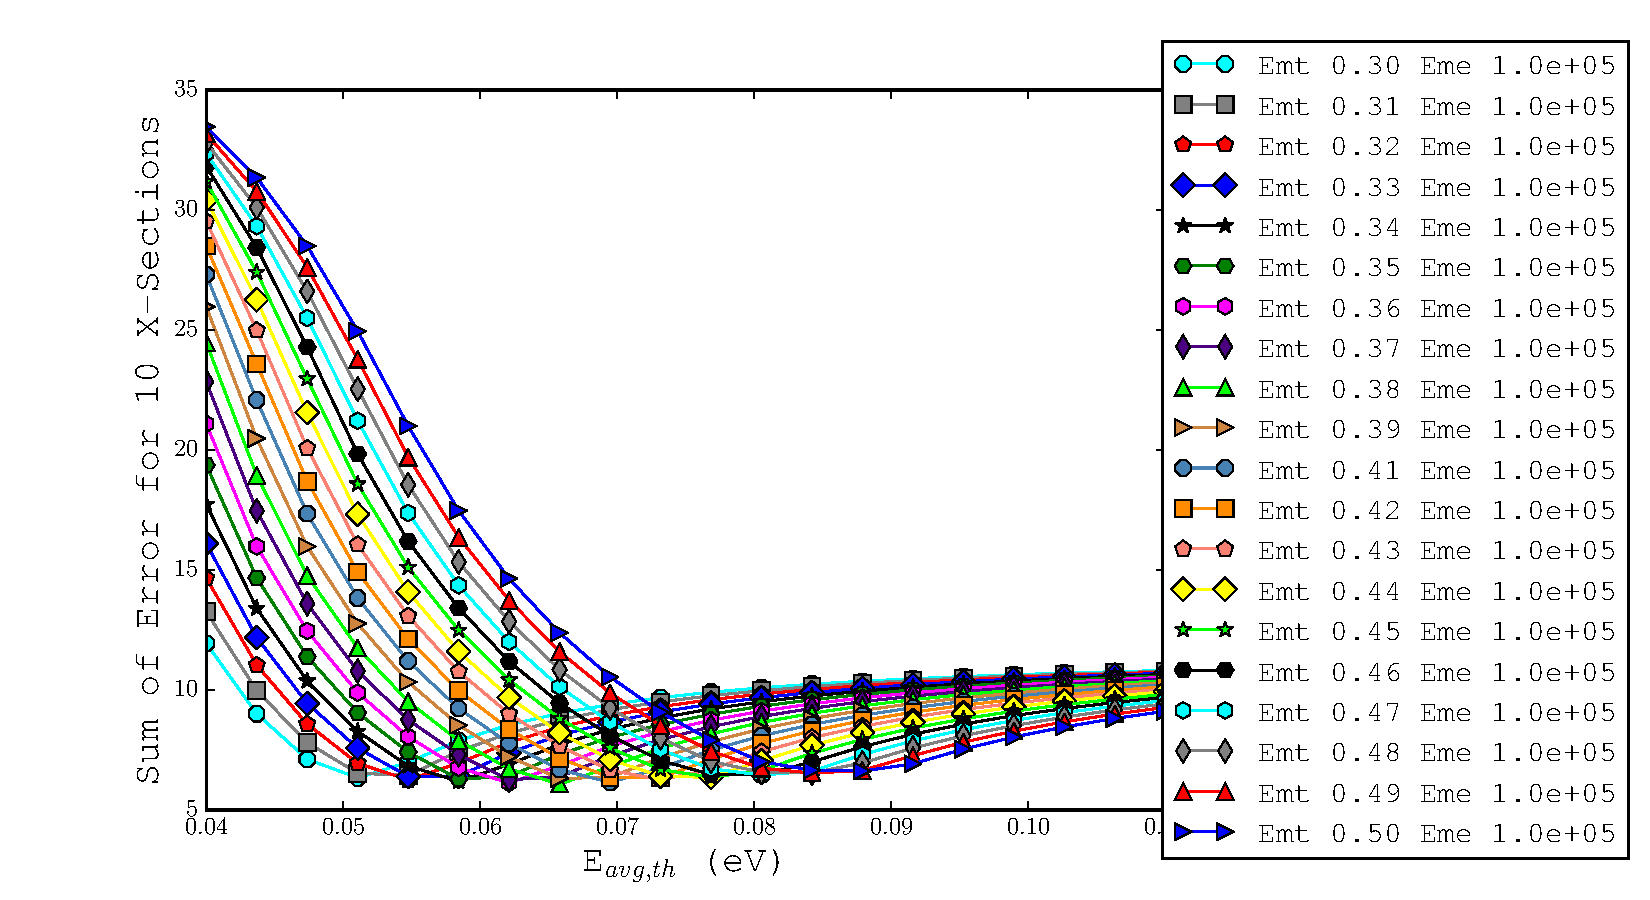
\includegraphics[width=0.9\columnwidth]{../Weighting/Reduce_Err/E0_vs_SumErr_third.pdf}
      \vspace{-5mm}
      \caption{Minimized error for 10 cross section calculations}
      \label{fig:err}
    \end{center}
  \end{figure}
  
  The flux spectrum is shown as below:

  \begin{figure}[H]
    \begin{center}
      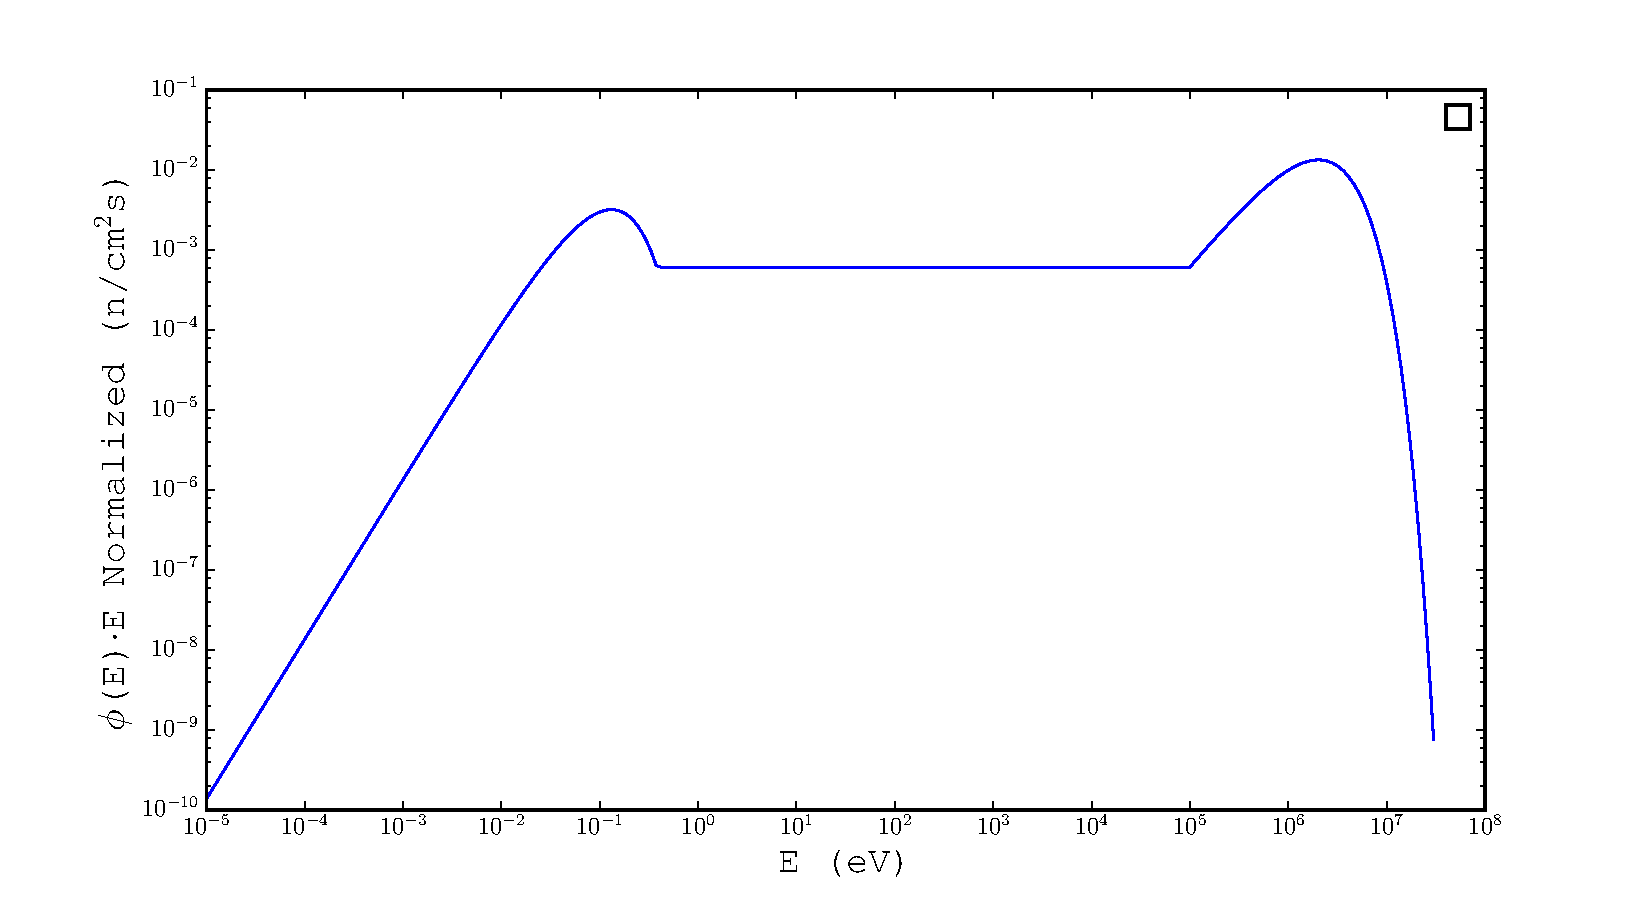
\includegraphics[width=0.9\columnwidth]{../Weighting/Flux_Spectra.pdf}
      \vspace{-5mm}
      \caption{Flux Spectra used for weighting x-sections and yields}
      \label{fig:Flux}
    \end{center}
  \end{figure}

  Table \ref{Table:3} shows the difference between my calculated cross
  section and the cross sections provided in ORIGEN2.
  The ratios will be used as a correction factor for the cross sections
  so that the input to ORIGEN2 will be constant.
  Differences
  have been attributed to the fact that the flux spectrum used
  does not capture reasonances. The cross sections were calculated
  with ENDF VII, and ORIGEN2 could have been processed with ENDF V,
  which would further account for differences, but has not been
  verified. The reason ENDF VII is being used for the current
  analysis is because the variance information is included
  in ENDF VII and not ENDF V.


  \begin{table}[H]
  \begin{center}
    \caption{Comparison of one-group cross sections}
    \label{Table:3}
    \begin{tabular}{l l l l}
      \toprule
      Isotope\tss{Rxn} & ENDF VII & ORIGEN2 & Ratio\\
      \hline
      \tss{239}Pu\tss{$\gamma$} & 6.544e+01 & 6.909E+01 & 1.06\\
      \tss{240}Pu\tss{$\gamma$} & 1.521e+02 & 2.228E+02 & 1.46\\
      \tss{241}Pu\tss{$\gamma$} & 4.518e+01 & 4.202E+01 & 0.93\\
      \tss{235}U\tss{$\gamma$}  & 9.387e+00 & 1.068E+01 & 1.14\\
      \tss{238}U\tss{$\gamma$}  & 4.098e+00 & 8.872E-01 & 0.22\\
      \tss{239}Pu\tss{f} & 1.179e+02 & 1.211E+02 & 1.03\\
      \tss{240}Pu\tss{f} & 9.609e-01 & 5.787E-01 & 0.60\\
      \tss{241}Pu\tss{f} & 1.253e+02 & 1.259E+02 & 1.01\\
      \tss{235}U\tss{f}  & 4.621e+01 & 4.752E+01 & 1.03\\
      \tss{238}U\tss{f}  & 2.091e-01 & 9.281E-02 & 0.44\\
      \bottomrule
    \end{tabular}
  \end{center}
  \end{table}

  Both $\sigma^{error}_\gamma$ and $\sigma^{error}_f$
  were determined by calculating the single group cross section
  with error subtracted, and then added. These values will
  constitue a mean with error. This was done with the following code:

  \pythonscript{../Weighting/Cal_Sig_w_Err}{Script calculating average x-sections}

  With results in Table \ref{Table:4}

  \begin{table}[H]
  \begin{center}
    \caption{Errors in single group cross sections}
    \label{Table:4}
    \begin{tabular}{l l}
      \toprule
      Isotope\tss{Rxn} & $\sigma$ with 1STD Error\\
      \hline
      \tss{239}Pu\tss{$\gamma$} & 69.09$\pm$8.15\\
      \tss{240}Pu\tss{$\gamma$} & 222.8$\pm$50.9\\
      \tss{241}Pu\tss{$\gamma$} & 42.02$\pm$10.92\\
      \tss{235}U\tss{$\gamma$}  & 10.68$\pm$3.23\\
      \tss{238}U\tss{$\gamma$}  & 0.887$\pm$0.175\\
      \tss{239}Pu\tss{f} & 121.1$\pm$1.2 \\
      \tss{240}Pu\tss{f} & 0.579$\pm$0.003 \\
      \tss{241}Pu\tss{f} & 125.9$\pm$2.3 \\
      \tss{235}U\tss{f}  & 47.52$\pm$0.71 \\
      \tss{238}U\tss{f}  & 0.093$\pm$8.2e-7 \\
      \bottomrule
    \end{tabular}
  \end{center}
  \end{table}


  
  Cross section versus flux for several isotopes are shown in the
  following figures.

  \begin{figure}[H]
    \begin{center}
      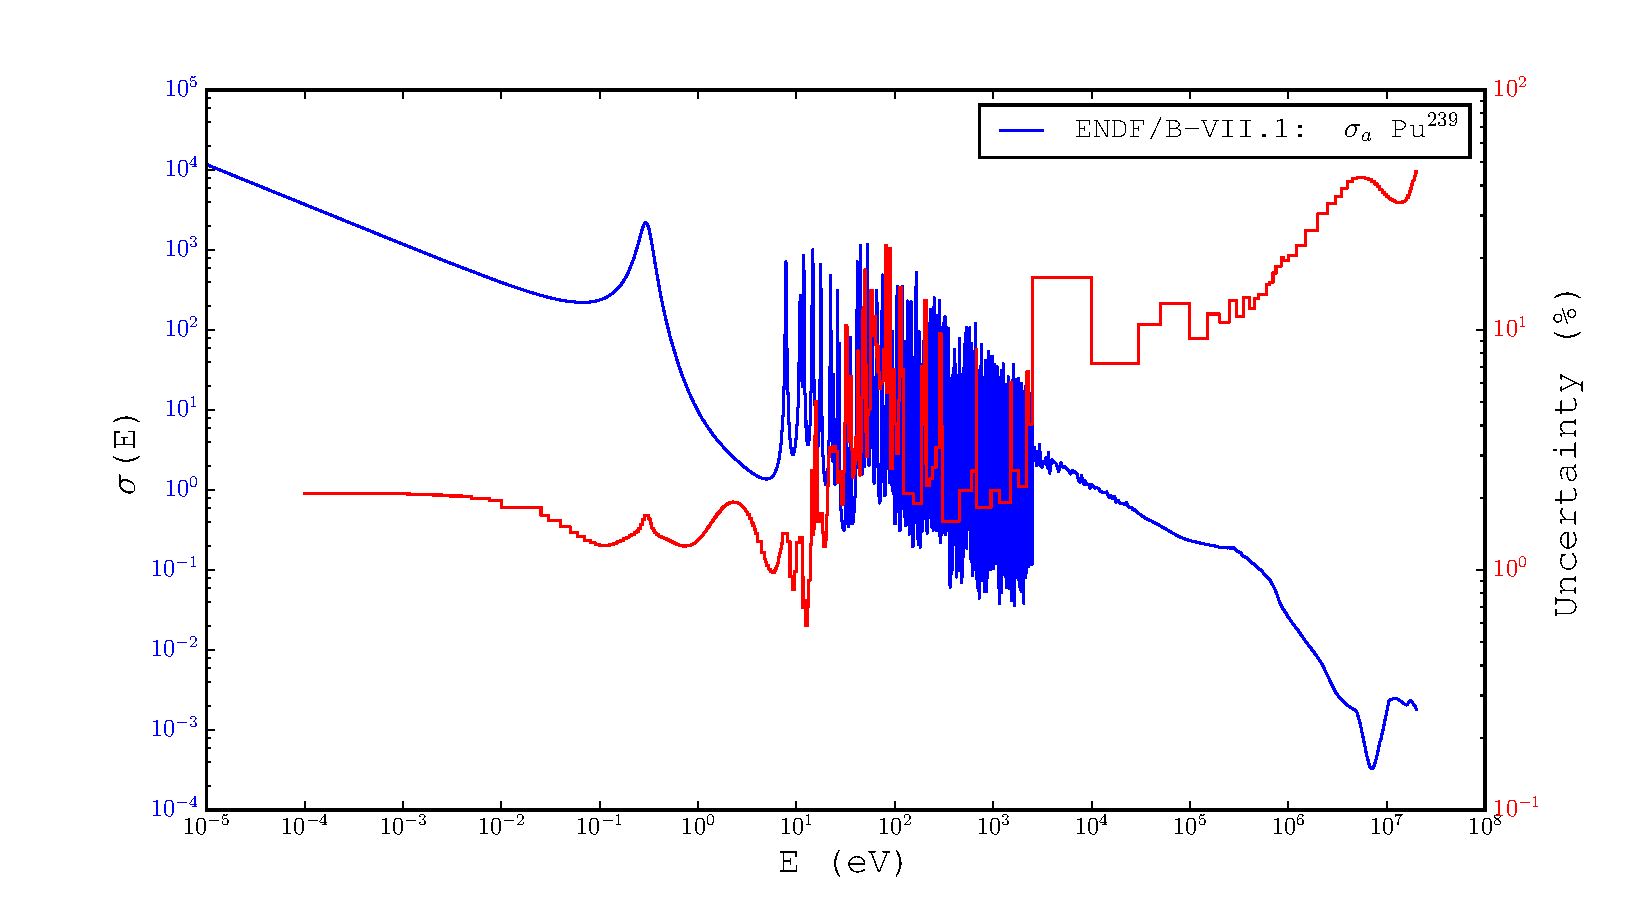
\includegraphics[width=0.9\columnwidth]{../Weighting/X_Sections/XwVar_Pu_239_94_a.pdf}
      \vspace{-5mm}
      \caption{$\sigma_a$ with corresponding error for \tss{239}Pu}
      \label{fig:XPu239}
    \end{center}
  \end{figure}

    \begin{figure}[H]
    \begin{center}
      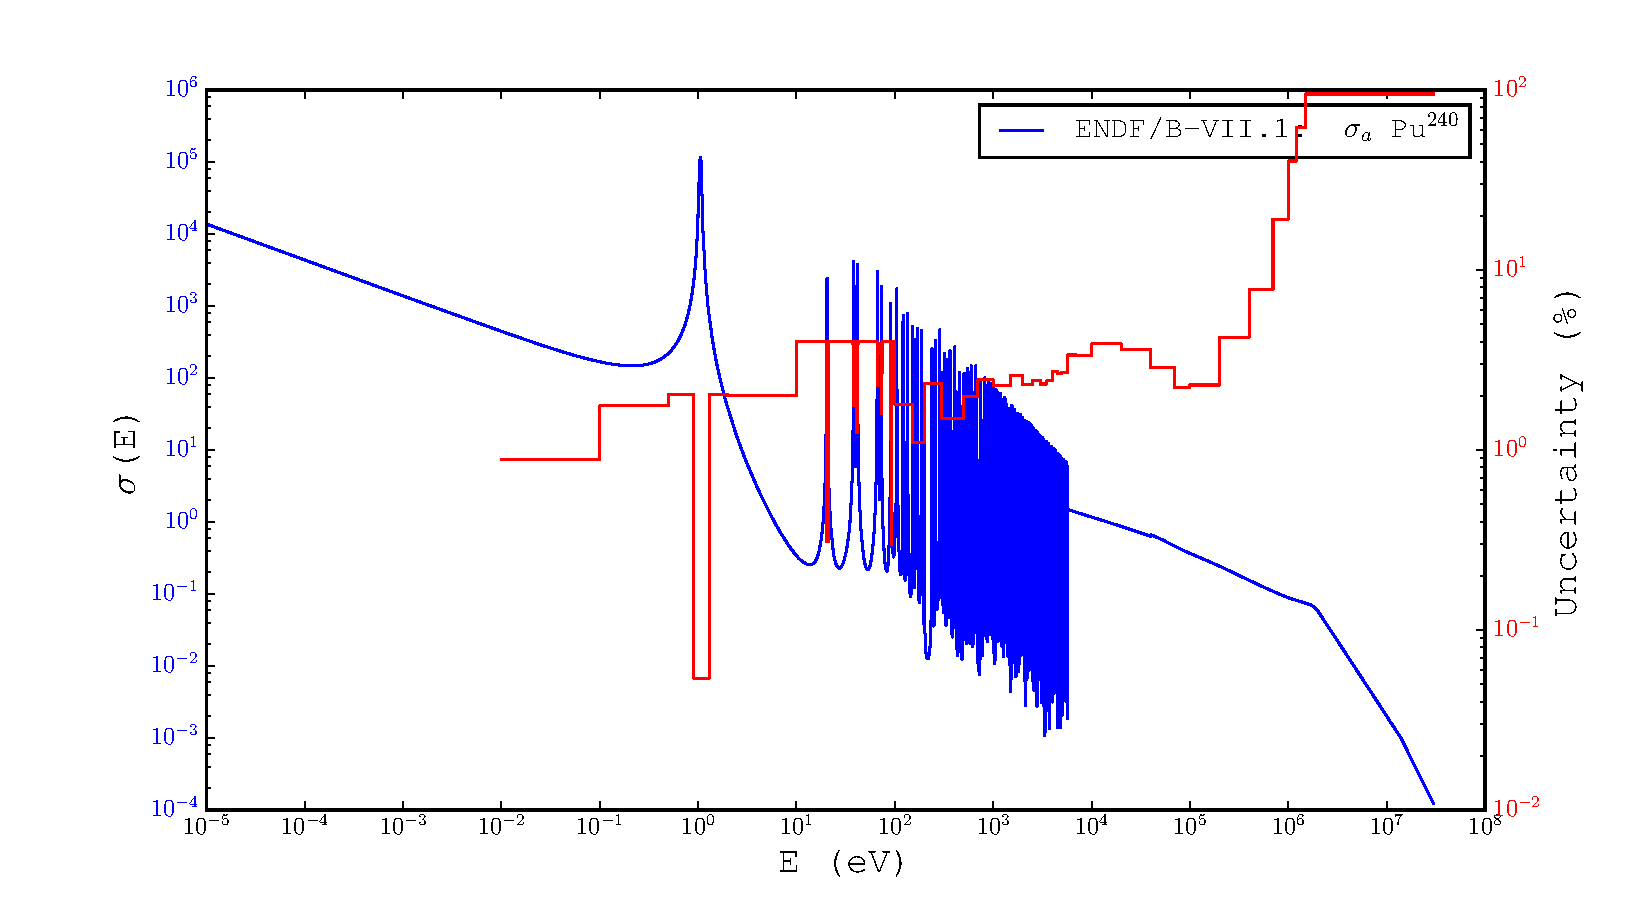
\includegraphics[width=0.9\columnwidth]{../Weighting/X_Sections/XwVar_Pu_240_94_a.pdf}
      \vspace{-5mm}
      \caption{$\sigma_a$ with corresponding error for \tss{240}Pu}
      \label{fig:XPu240}
    \end{center}
  \end{figure}

    \begin{figure}[H]
    \begin{center}
      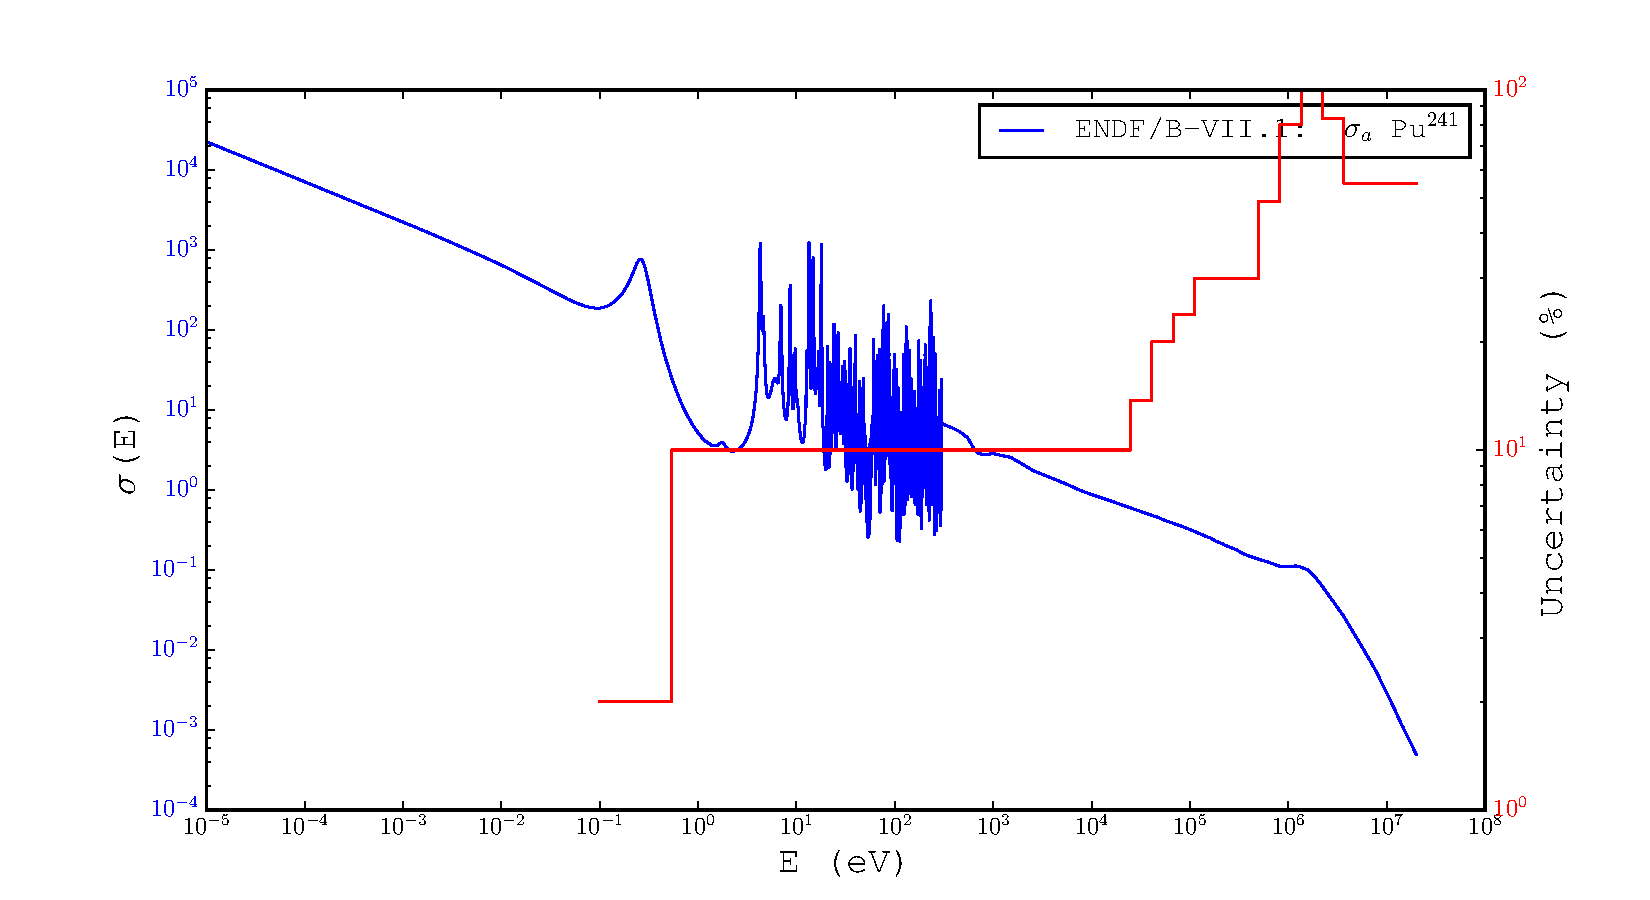
\includegraphics[width=0.9\columnwidth]{../Weighting/X_Sections/XwVar_Pu_241_94_a.pdf}
      \vspace{-5mm}
      \caption{$\sigma_a$ with corresponding error for \tss{241}Pu}
      \label{fig:XPu241}
    \end{center}
  \end{figure}

  \begin{figure}[H]
    \begin{center}
      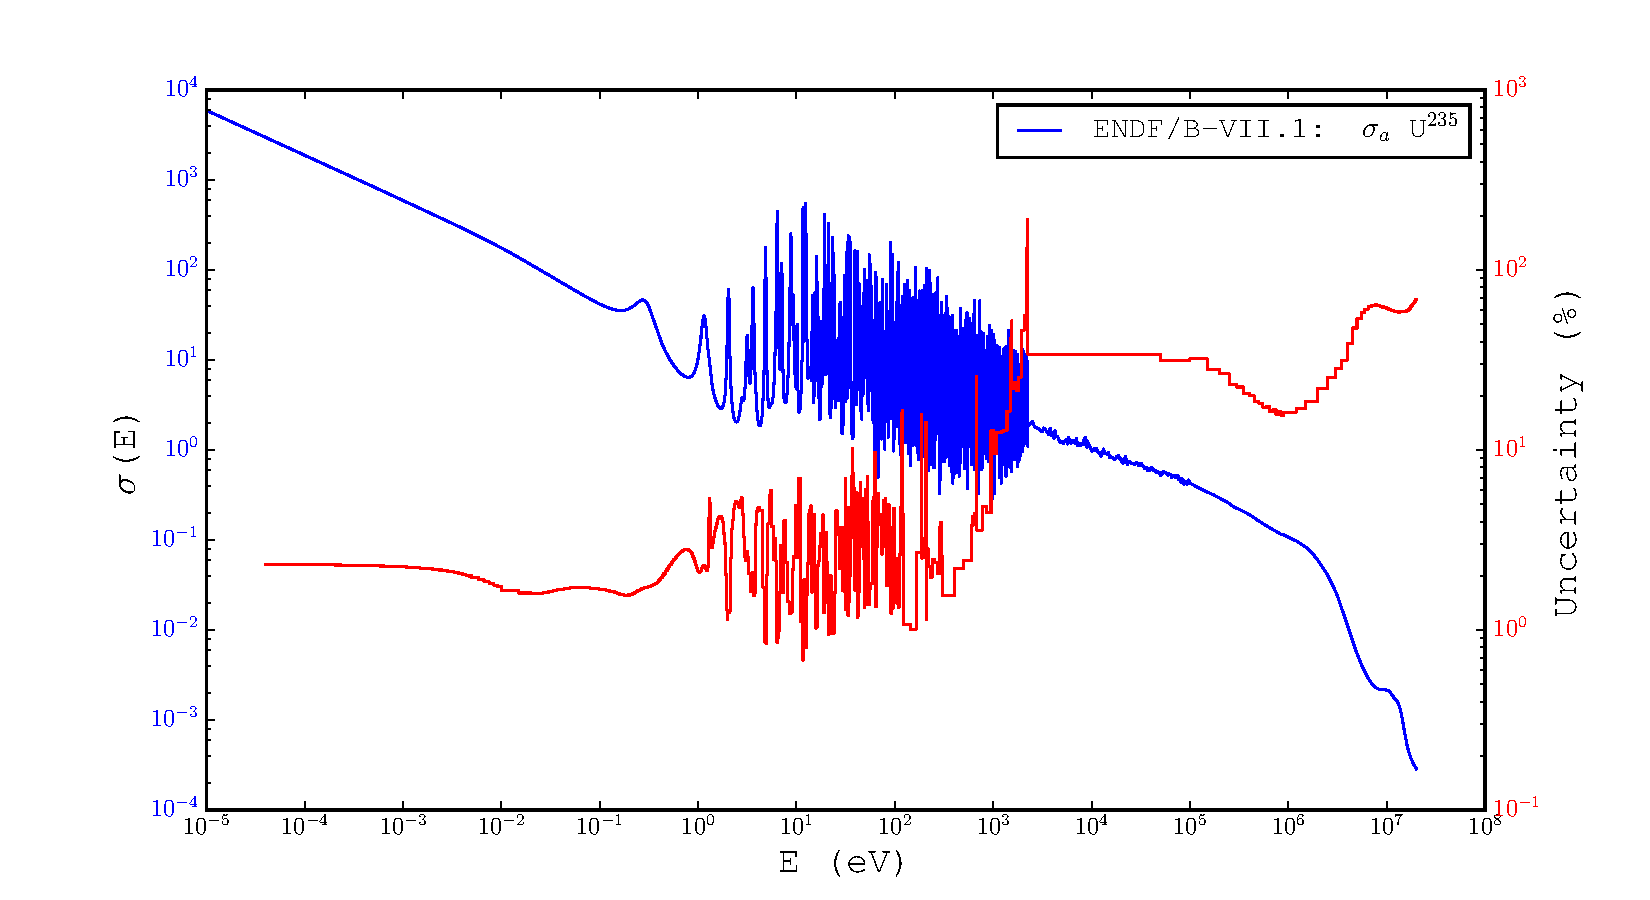
\includegraphics[width=0.9\columnwidth]{../Weighting/X_Sections/XwVar_U_235_92_a.pdf}
      \vspace{-5mm}
      \caption{$\sigma_a$ with corresponding error for \tss{235}U}
      \label{fig:XU235}
    \end{center}
  \end{figure}

  \begin{figure}[H]
    \begin{center}
      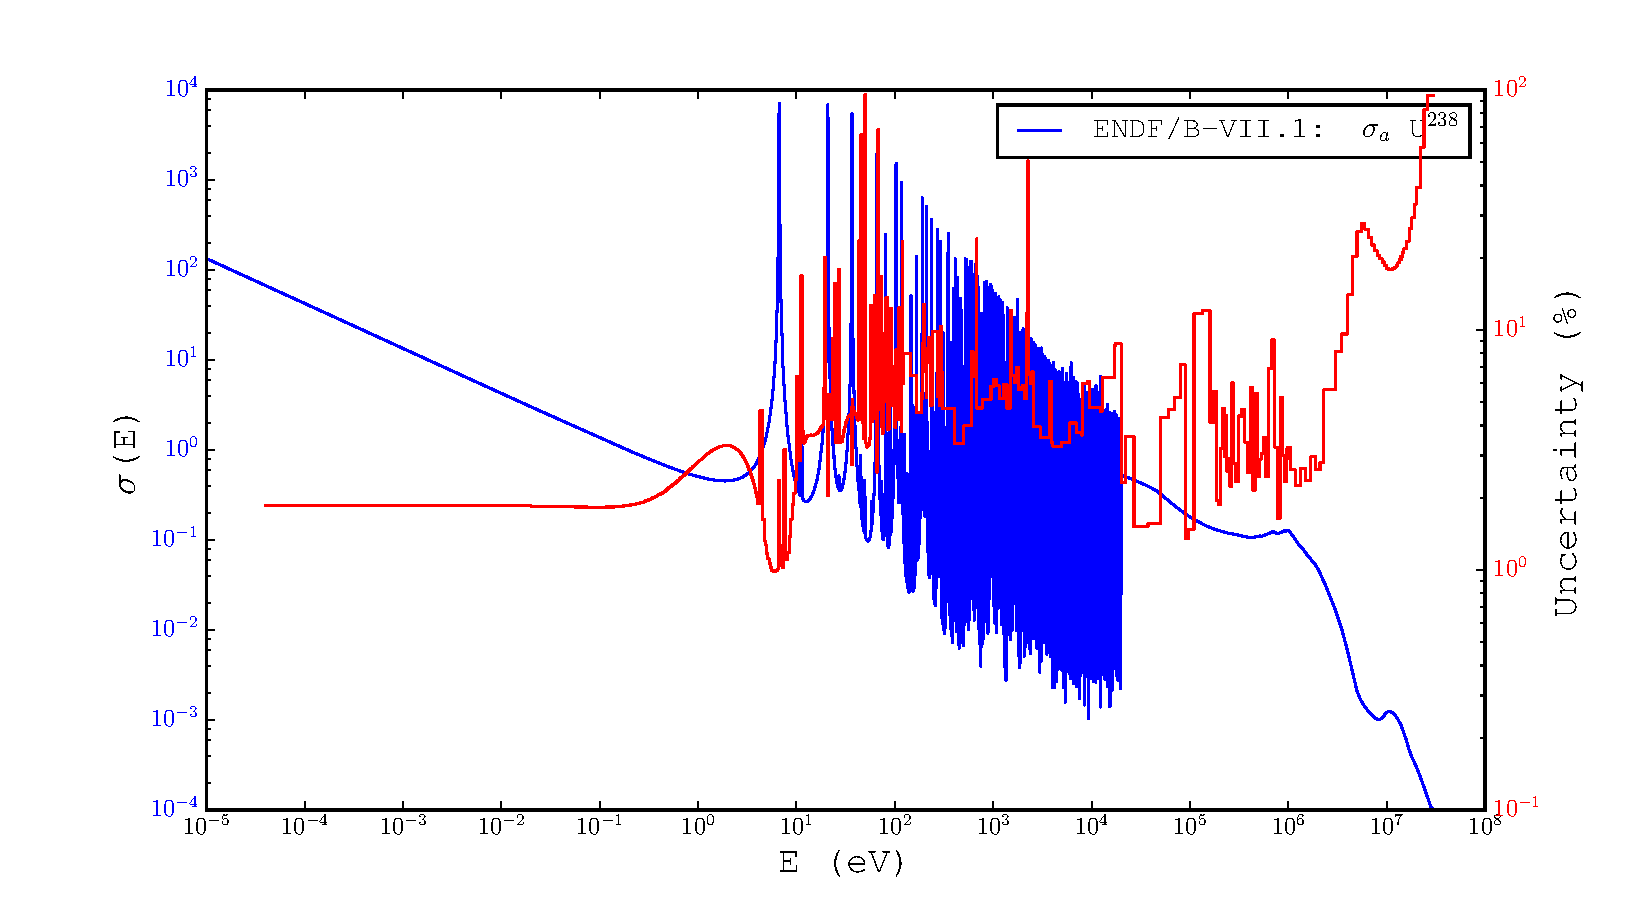
\includegraphics[width=0.9\columnwidth]{../Weighting/X_Sections/XwVar_U_238_92_a.pdf}
      \vspace{-5mm}
      \caption{$\sigma_a$ with corresponding error for \tss{238}U}
      \label{fig:XU238}
    \end{center}
  \end{figure}

  \begin{figure}[H]
    \begin{center}
      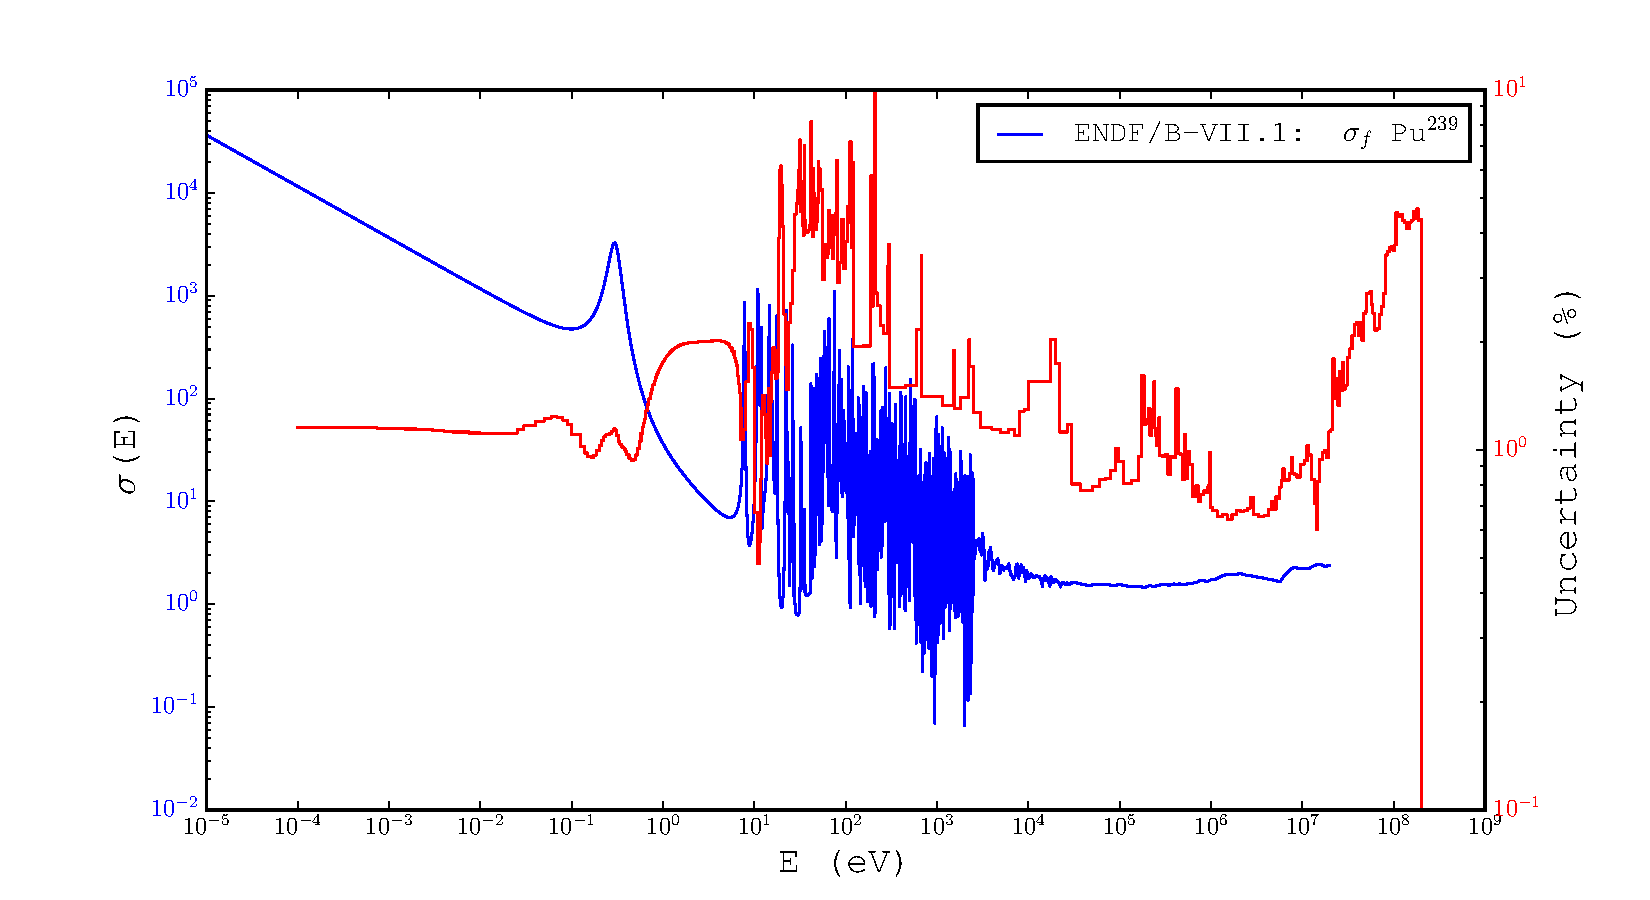
\includegraphics[width=0.9\columnwidth]{../Weighting/X_Sections/XwVar_Pu_239_94_f.pdf}
      \vspace{-5mm}
      \caption{$\sigma_f$ with corresponding error for \tss{239}Pu}
      \label{fig:XPu239}
    \end{center}
  \end{figure}

    \begin{figure}[H]
    \begin{center}
      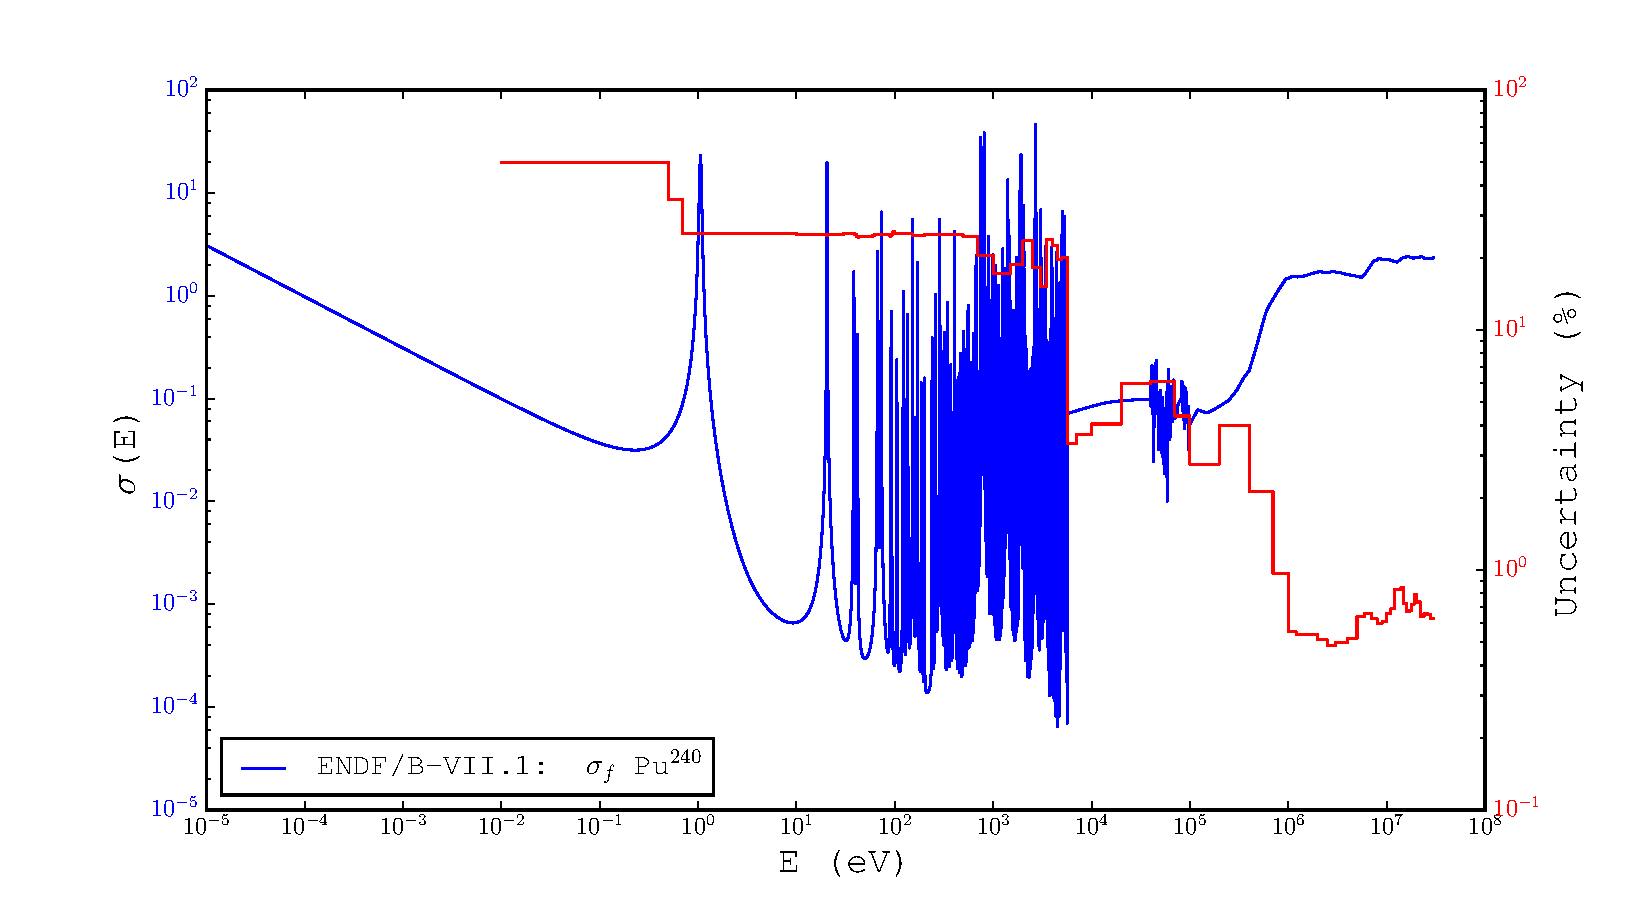
\includegraphics[width=0.9\columnwidth]{../Weighting/X_Sections/XwVar_Pu_240_94_f.pdf}
      \vspace{-5mm}
      \caption{$\sigma_f$ with corresponding error for \tss{240}Pu}
      \label{fig:XPu240}
    \end{center}
  \end{figure}

    \begin{figure}[H]
    \begin{center}
      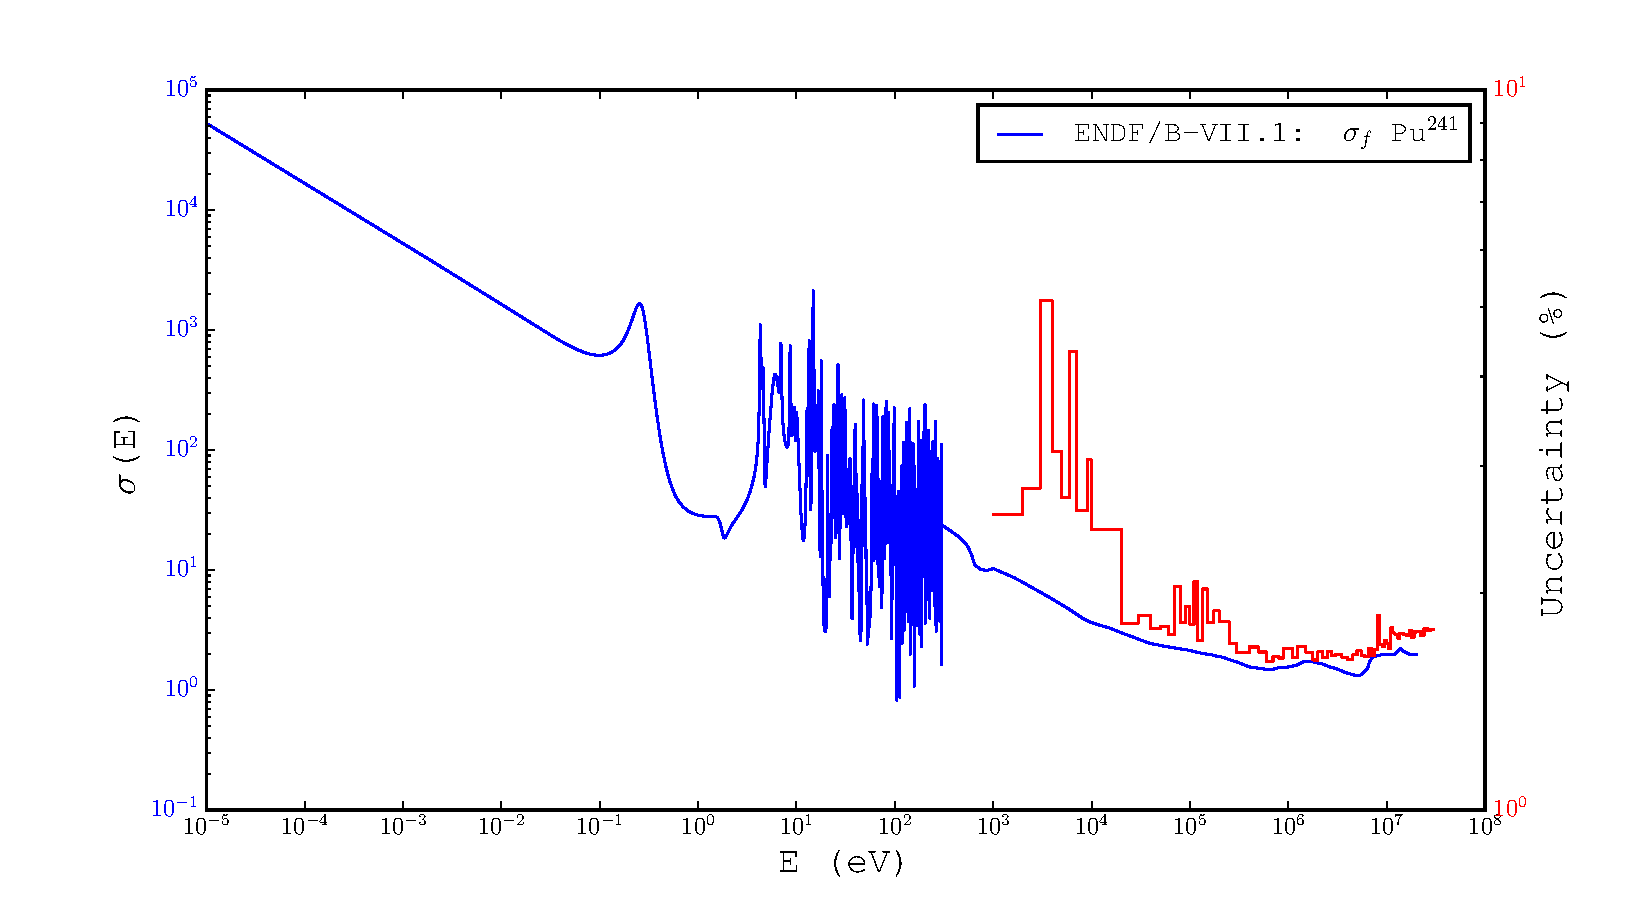
\includegraphics[width=0.9\columnwidth]{../Weighting/X_Sections/XwVar_Pu_241_94_f.pdf}
      \vspace{-5mm}
      \caption{$\sigma_f$ with corresponding error for \tss{241}Pu}
      \label{fig:XPu241}
    \end{center}
  \end{figure}

  \begin{figure}[H]
    \begin{center}
      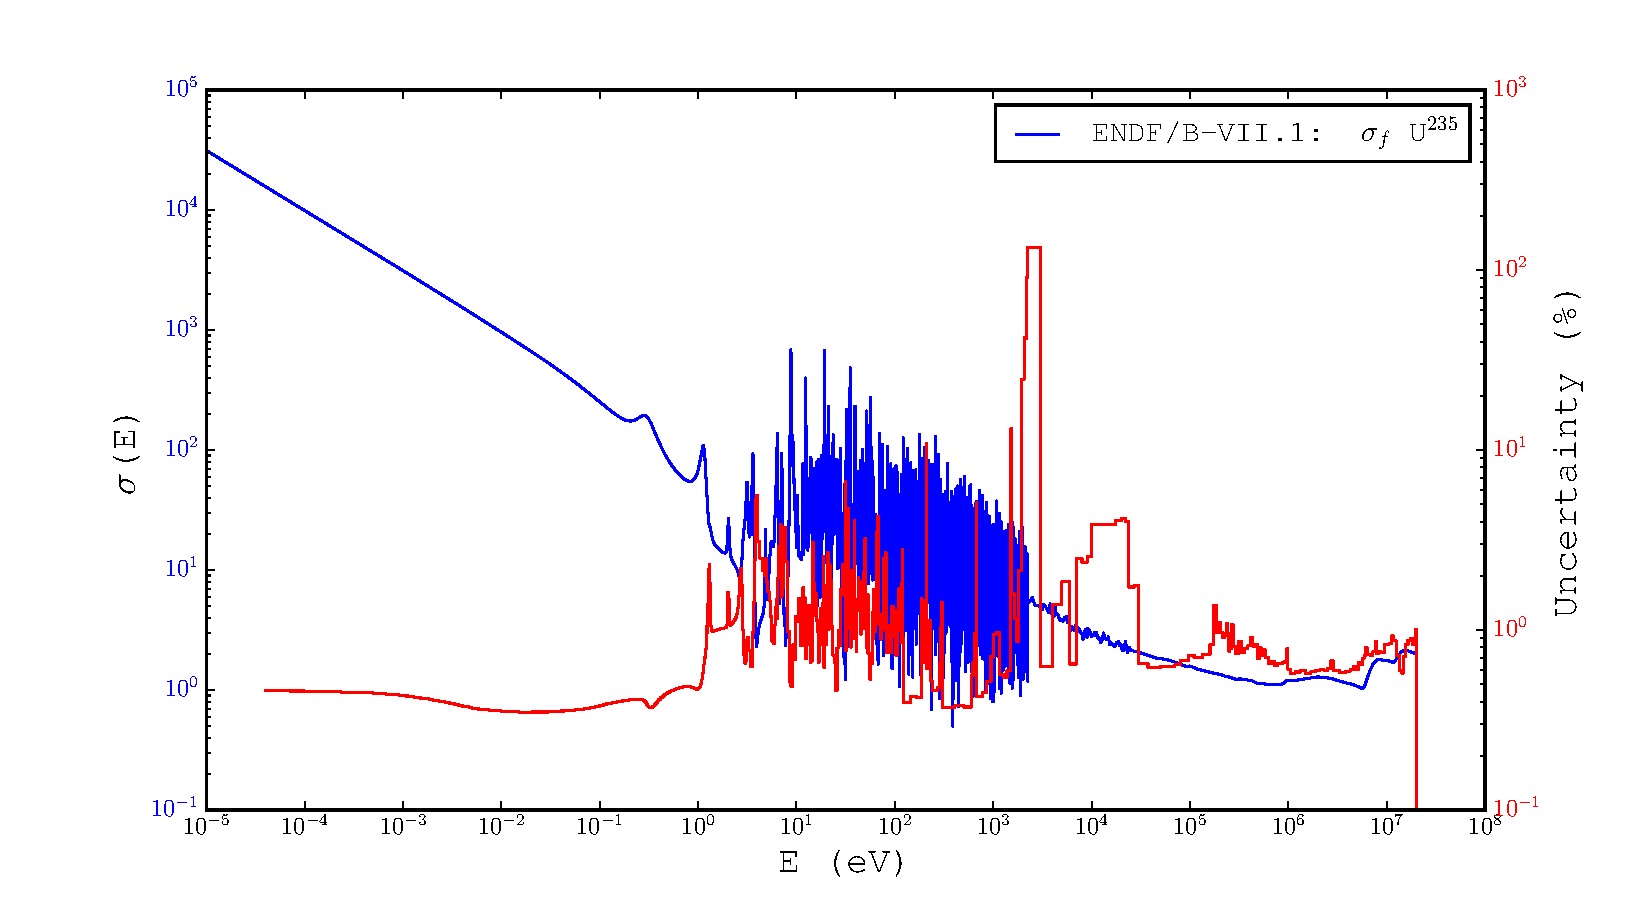
\includegraphics[width=0.9\columnwidth]{../Weighting/X_Sections/XwVar_U_235_92_f.pdf}
      \vspace{-5mm}
      \caption{$\sigma_f$ with corresponding error for \tss{235}U}
      \label{fig:XU235}
    \end{center}
  \end{figure}

  \begin{figure}[H]
    \begin{center}
      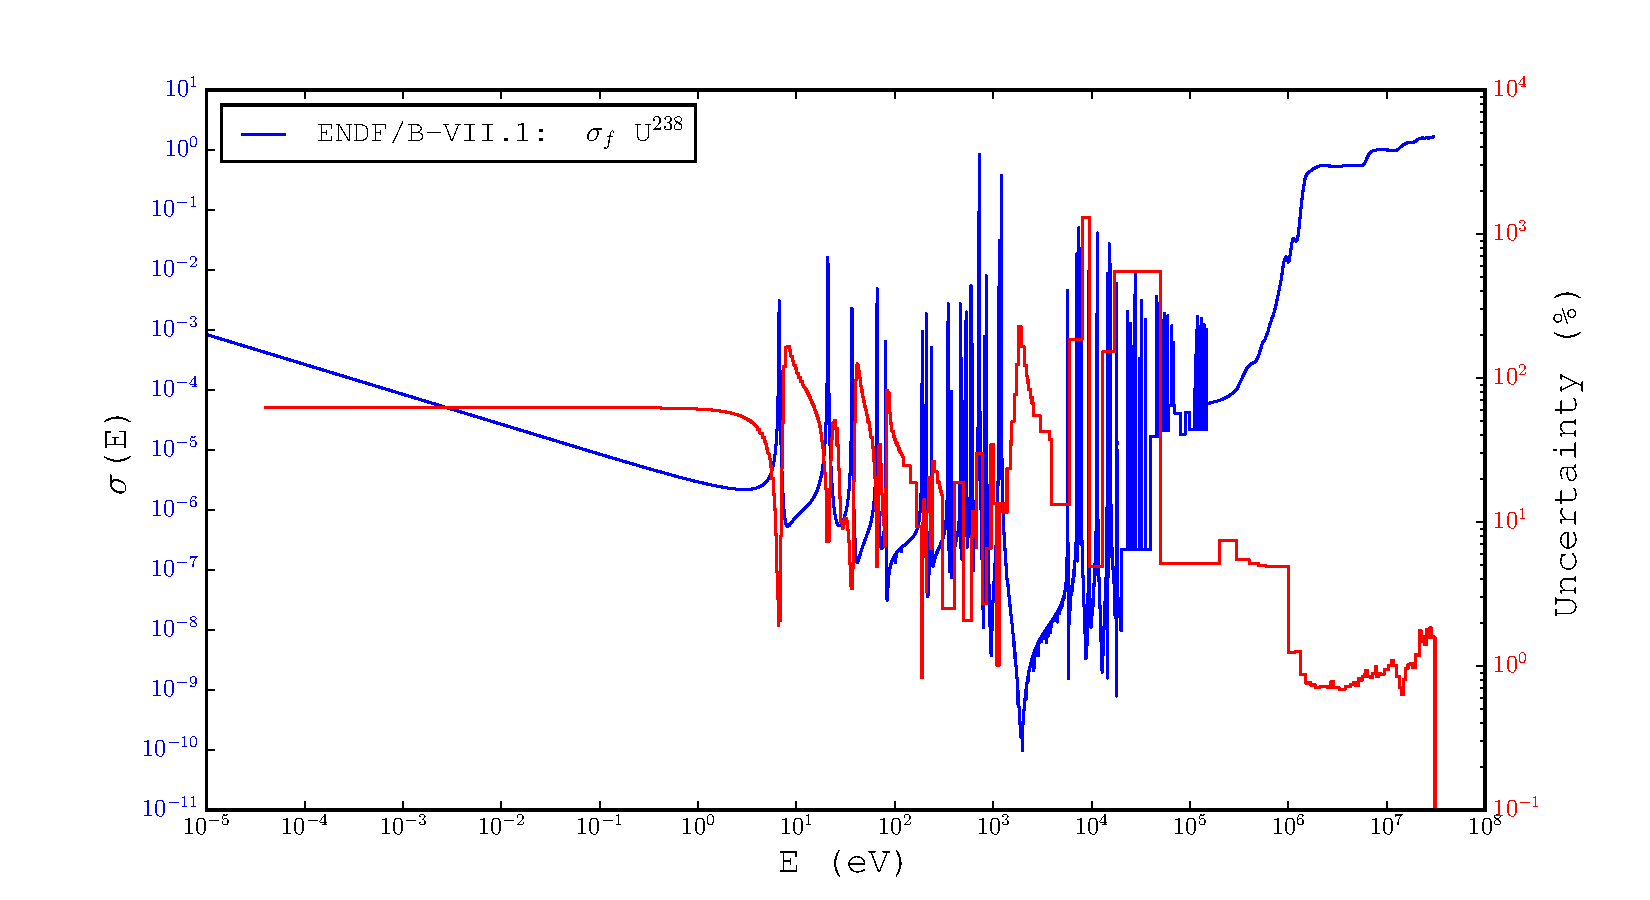
\includegraphics[width=0.9\columnwidth]{../Weighting/X_Sections/XwVar_U_238_92_f.pdf}
      \vspace{-5mm}
      \caption{$\sigma_f$ with corresponding error for \tss{238}U}
      \label{fig:XU238}
    \end{center}
  \end{figure}

  
    
\item[\done]{Create a sampling space for all possible variations of
  calculations}

  The distribution for all 10 of the above cross sections are
  assumed as Gamma distributions to avoid negative cross section
  values.
  \begin{equation*}
    \pi(\theta)=\frac{\theta^{\alpha-1}e^{-\theta/\beta}}{\Gamma(\alpha)
      \beta^{\alpha}},\ \ \ \ \ \theta,\alpha,\beta>0.
  \end{equation*}
  Therefore, we say that $\theta\sim G(\alpha,\beta)$. Where the mean
  and errors determined above fit into $\alpha$ and $\beta$ via
  \begin{equation*}
    \alpha=\frac{\text{Mean}^2}{\text{Error}^2}
  \end{equation*}
  and
  \begin{equation*}
    \beta=\frac{\text{Error}^2}{\text{Mean}}
  \end{equation*}
  
  
  With the following codes the sampling space was detemined.

  
  \pythonscript{../Origen2/SampleGen}{Sample Generation code}


  Below are histograms of the sampling space, most of the others look
  the same, with samples surrounding the mean.
  
  \begin{figure}[H]
    \begin{center}
      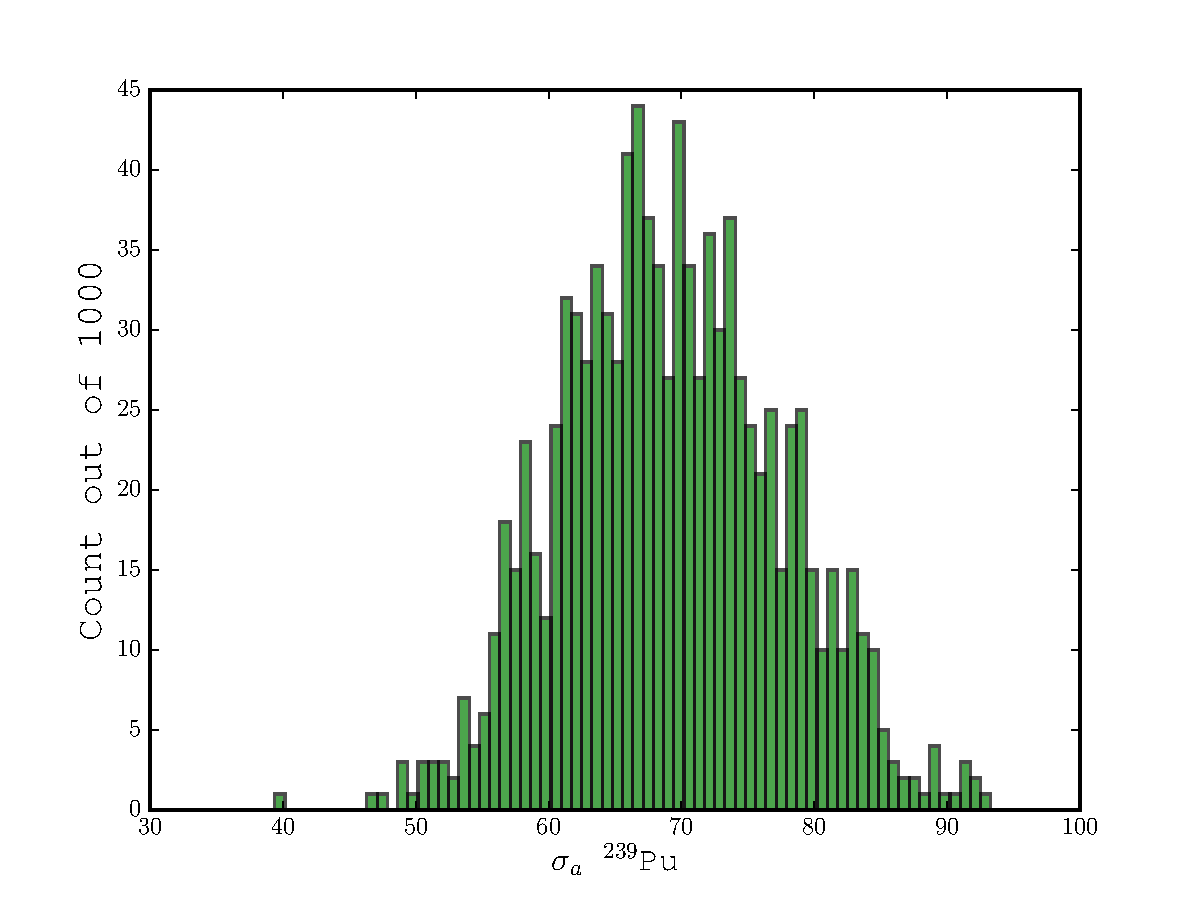
\includegraphics[width=0.77\columnwidth]{../Origen2/PLOTS/94Pu239aHIST.pdf}
      \vspace{-5mm}
      \caption{Histogram of sample space for $\sigma_a$ \tss{239}Pu}
      \label{fig:SPu239a}
    \end{center}
  \end{figure}

  \begin{figure}[H]
    \begin{center}
      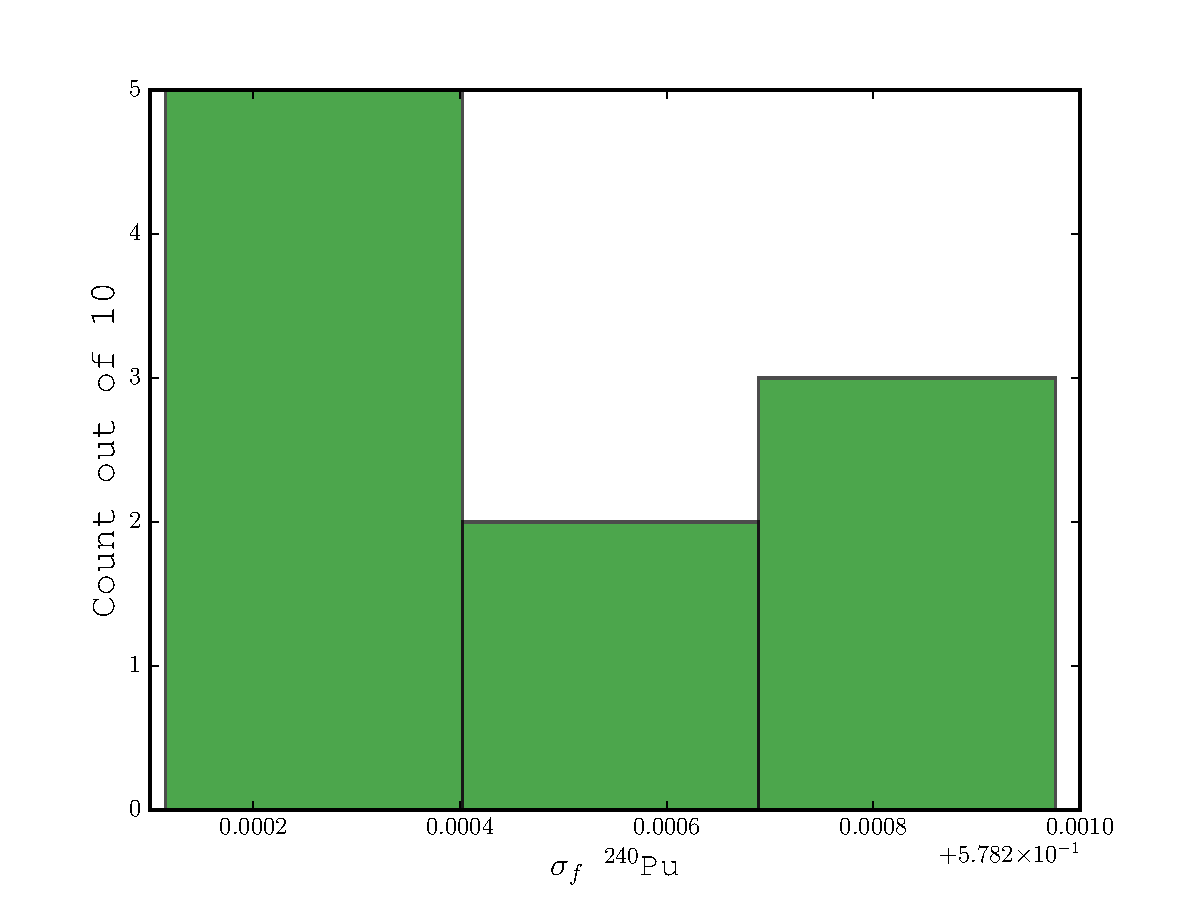
\includegraphics[width=0.77\columnwidth]{../Origen2/PLOTS/94Pu240fHIST.pdf}
      \vspace{-5mm}
      \caption{Histogram of sample space for $\sigma_f$ \tss{240}Pu}
      \label{fig:SPu240f}
    \end{center}
  \end{figure}


  The sampling spaces were run through ORIGEN with the code
  shown in the first section.
  
  
  %% I might have to reduce the number of elements to look at,
  %% maybe I'll start by
  %% just looking at \tss{154}Eu.
  %% \begin{equation*}
  %%   ^{153}Pm\xrightarrow{\beta^-} {^{153}Sm}\xrightarrow{\beta^-}
  %%   {^{153}Eu}
  %%   \xrightarrow{(n,\gamma)} {^{154}Eu}
  %% \end{equation*}

  %% \begin{table}[H]
  %% \begin{center}
  %%   \caption{Summary of parameters to vary for \tss{154}Eu}
  %%   \label{Table:4}
  %%   \begin{tabular}{l|l|l|l}
  %%     \toprule
  %%     Isotope & Half-life & $\sigma_\gamma$ & Yield\\
  %%     \hline
  %%     \tss{153}Pm & 5.25 $\pm$ 0.02 min & SIGMA & Yield \\
  %%     \tss{153}Sm & 46.284 $\pm$ 0.004 hr & SIGMA & Yield\\
  %%     \tss{153}Eu & Stable & SIGMA & Yield \\
  %%     \tss{154}Eu & 8.60 $\pm$ 0.01 y  & SIGMA & Yield \\
  %%     \bottomrule
  %%   \end{tabular}
  %% \end{center}
  %% \end{table}

  
\item[\done]{Plot Results}

  The function for plotting results are shown below.

  \pythonscript{../Origen2/PLOToutput}{Code for plots}

  
\end{todolist}


%------------------------------------------------------------
%	Quantities of Interest and uncertain parameters
%------------------------------------------------------------

\section{Results}

Quantities of interest are shown in Table \ref{Table:1} above.
The uncertain parameters were the absorption and fission
cross-sections for \tss{235}U, \tss{238}U, \tss{239}Pu,
\tss{240}Pu, and \tss{241}Pu.

Results are graphically represented below. 

  \begin{figure}[H]
    \begin{center}
      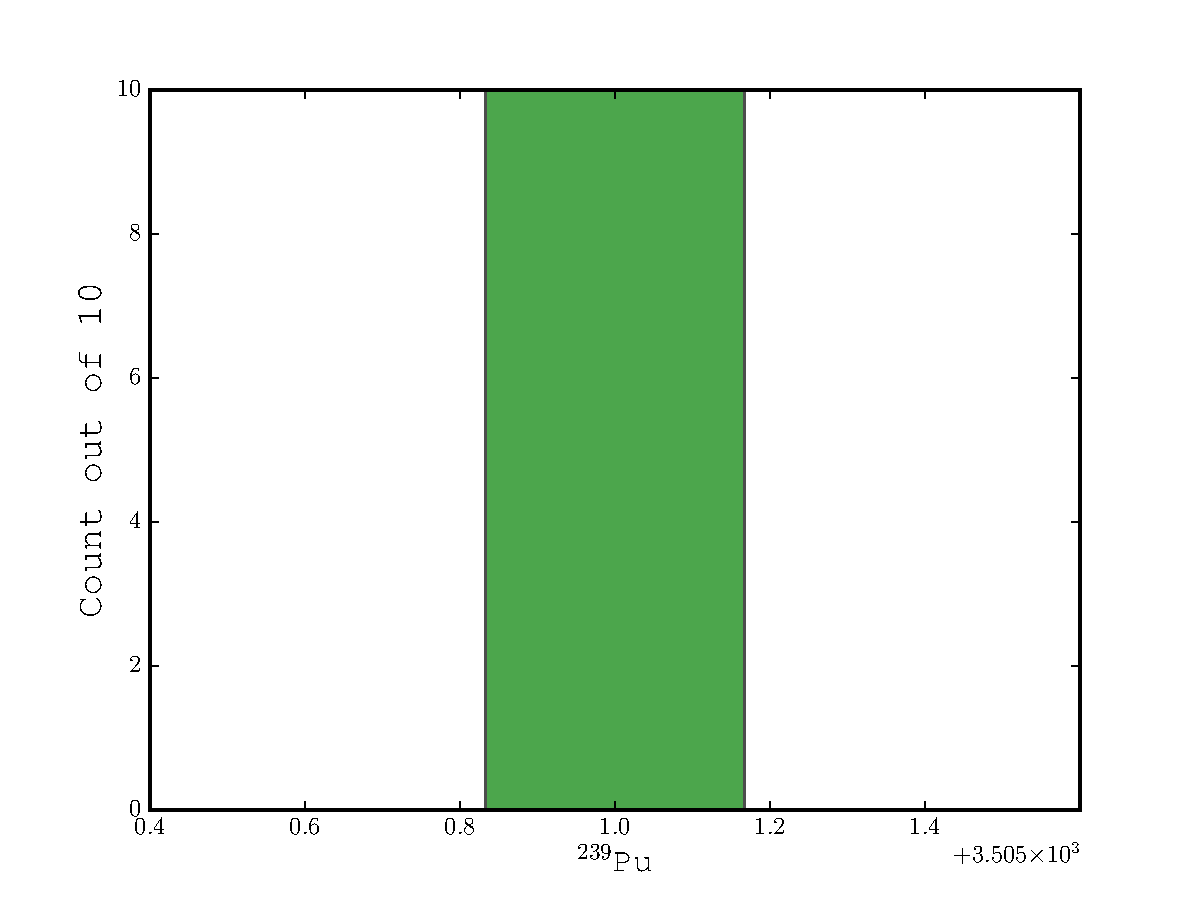
\includegraphics[width=0.77\columnwidth]{../Origen2/PLOTS/PU239Post_HIST.pdf}
      \vspace{-5mm}
      \caption{Histogram of QOI \tss{239}Pu}
      \label{fig:POSTHISTPu239}
    \end{center}
  \end{figure}

    \begin{figure}[H]
    \begin{center}
      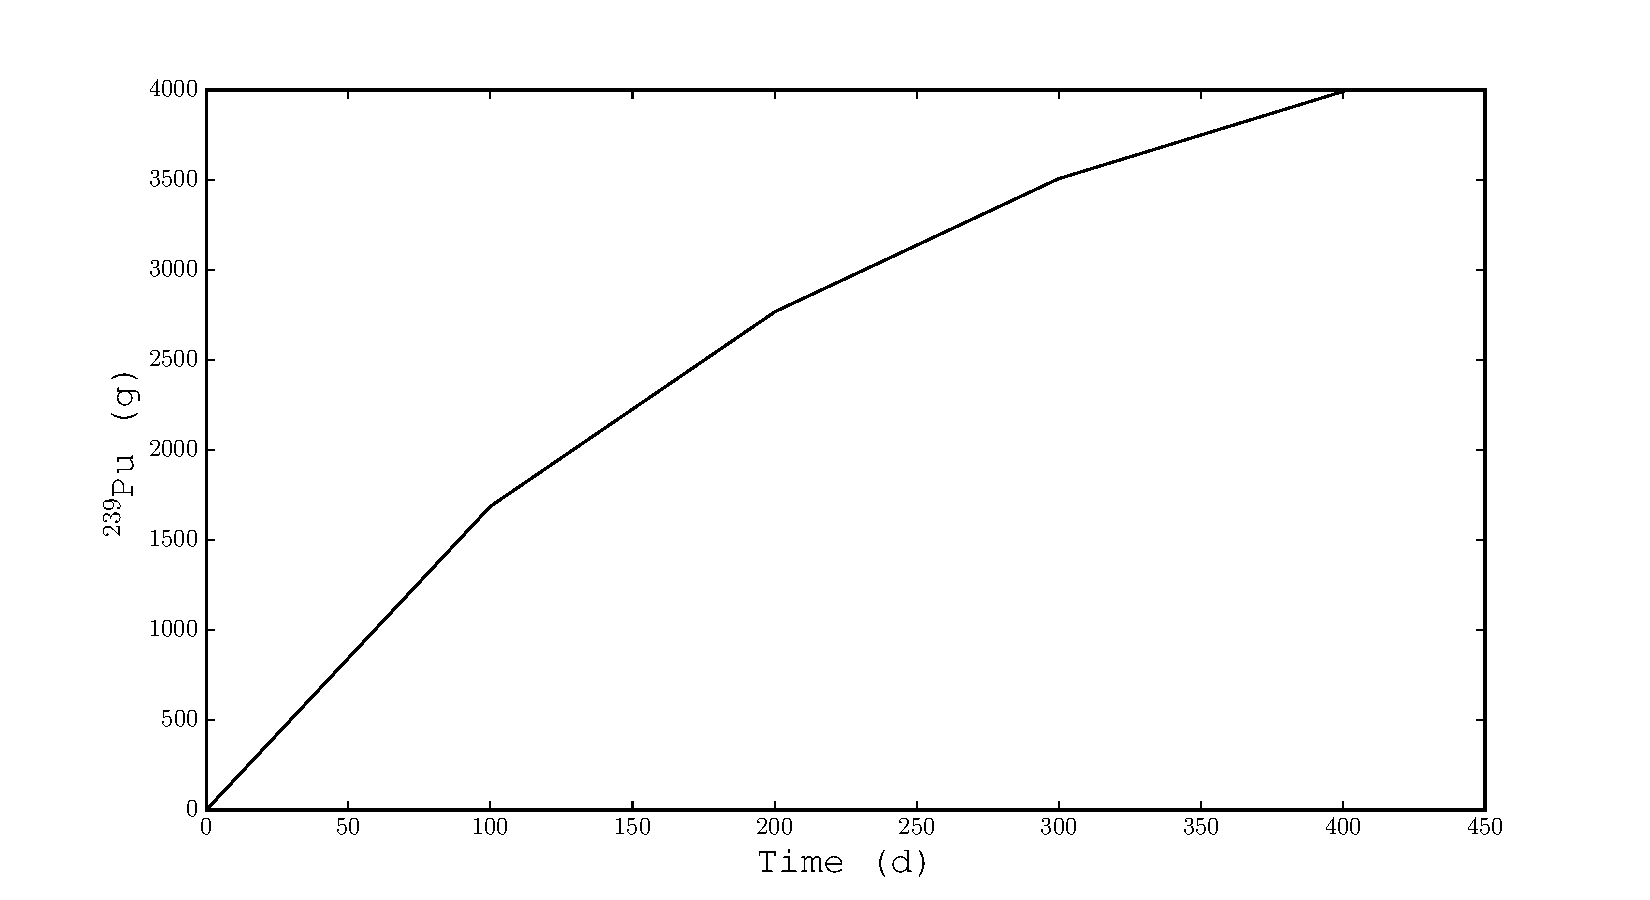
\includegraphics[width=0.77\columnwidth]{../Origen2/PLOTS/PU239Post_XY.pdf}
      \vspace{-5mm}
      \caption{XY plot of QOI \tss{239}Pu}
      \label{fig:POSTXYPu239}
    \end{center}
  \end{figure}


  \begin{figure}[H]
    \begin{center}
      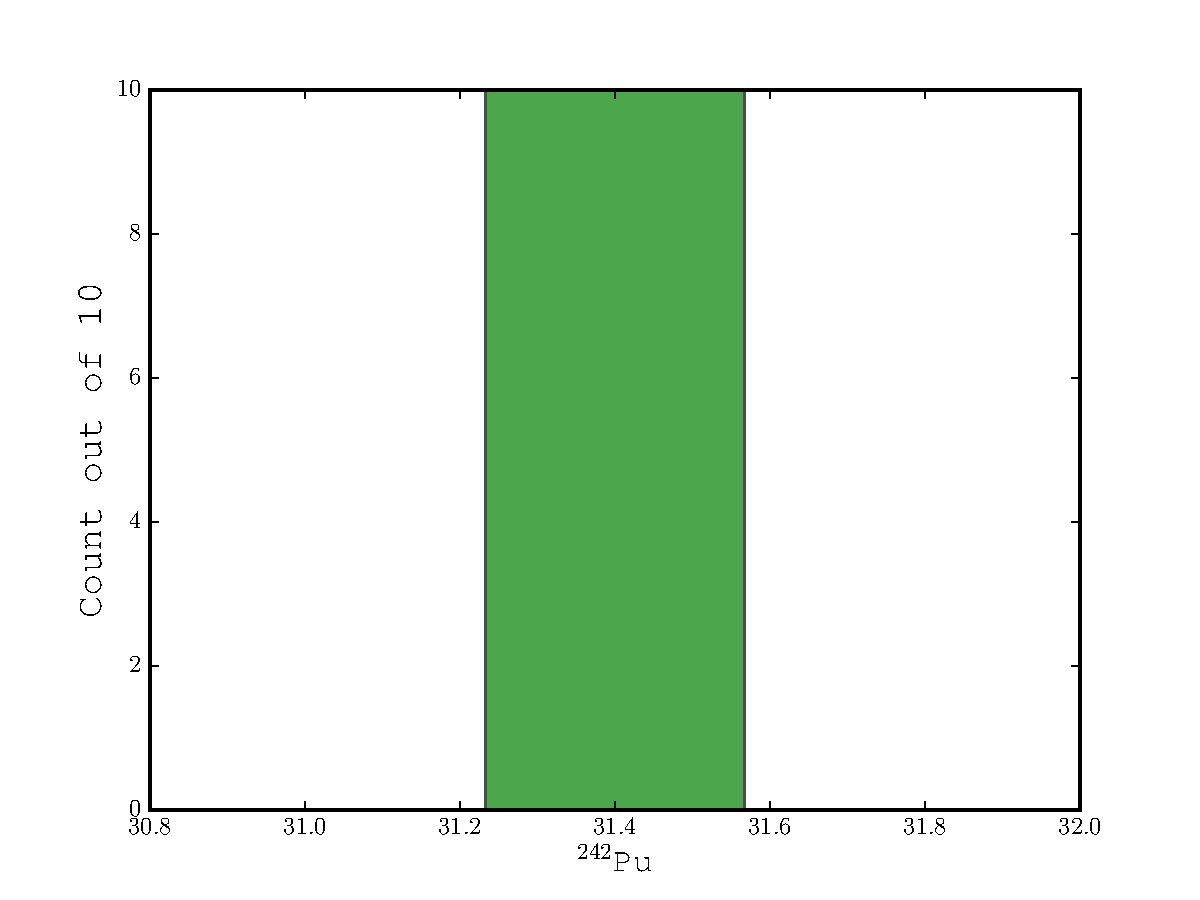
\includegraphics[width=0.77\columnwidth]{../Origen2/PLOTS/PU242Post_HIST.pdf}
      \vspace{-5mm}
      \caption{Histogram of QOI \tss{242}Pu}
      \label{fig:POSTHISTPu242}
    \end{center}
  \end{figure}

    \begin{figure}[H]
    \begin{center}
      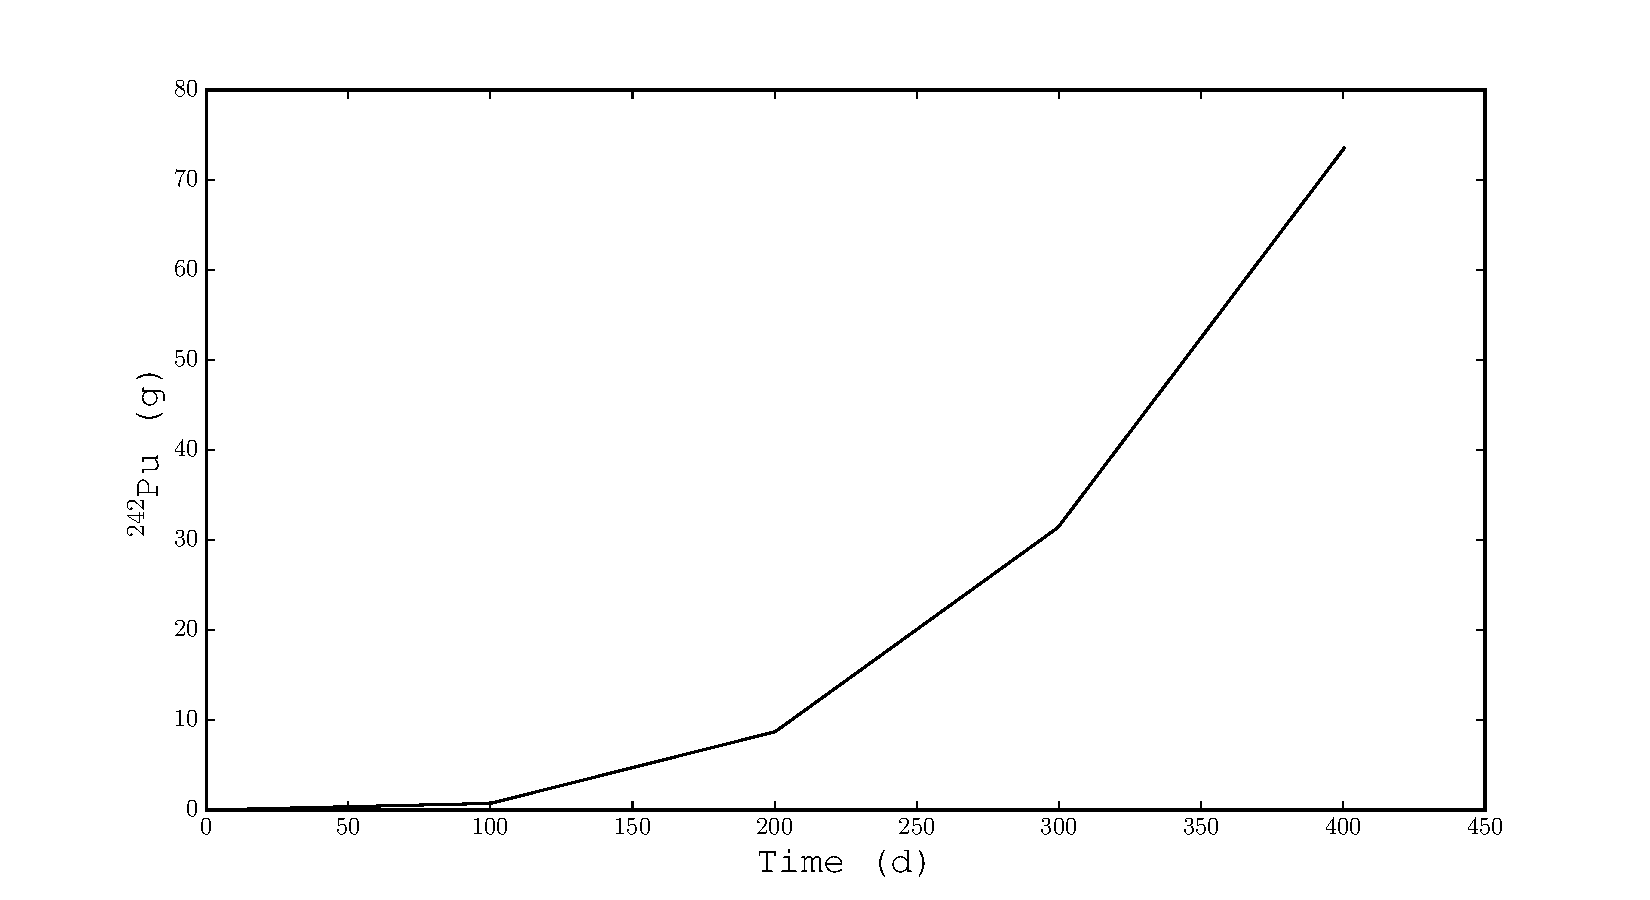
\includegraphics[width=0.77\columnwidth]{../Origen2/PLOTS/PU242Post_XY.pdf}
      \vspace{-5mm}
      \caption{XY plot of QOI \tss{242}Pu}
      \label{fig:POSTXYPu242}
    \end{center}
  \end{figure}

  \begin{figure}[H]
    \begin{center}
      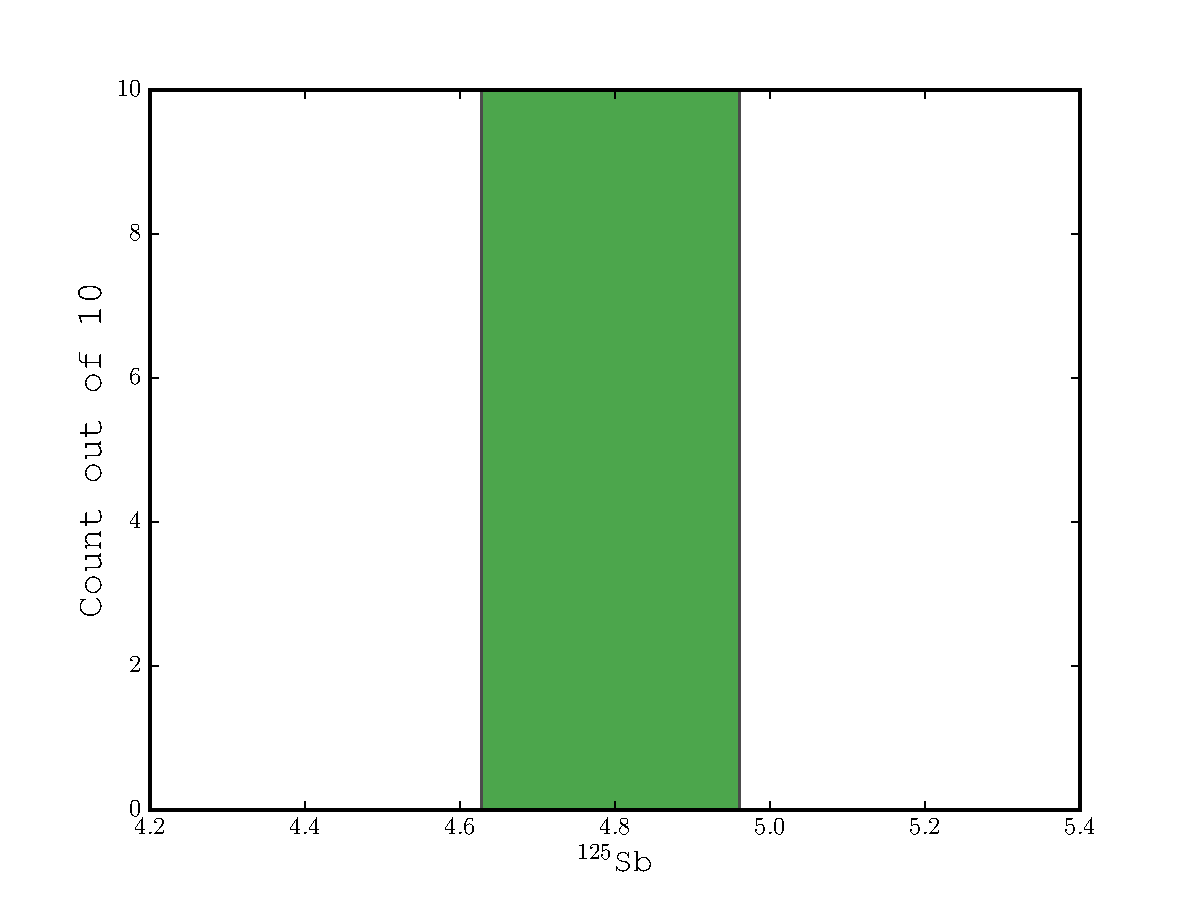
\includegraphics[width=0.77\columnwidth]{../Origen2/PLOTS/SB125Post_HIST.pdf}
      \vspace{-5mm}
      \caption{Histogram of QOI \tss{125}Sb}
      \label{fig:POSTHISTSb125}
    \end{center}
  \end{figure}

    \begin{figure}[H]
    \begin{center}
      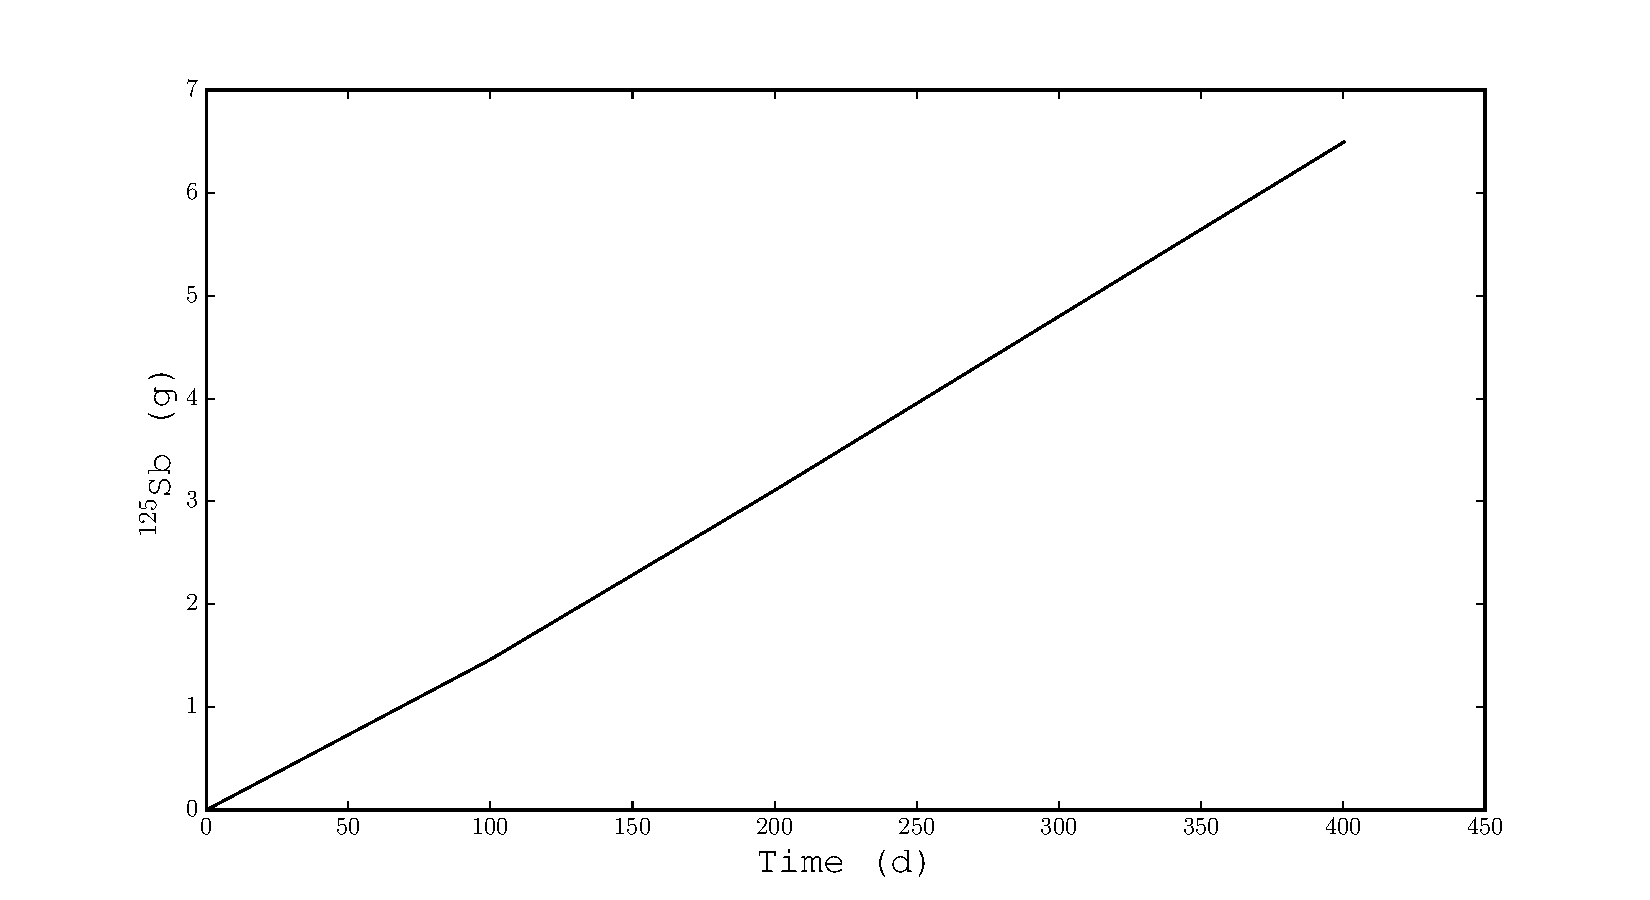
\includegraphics[width=0.77\columnwidth]{../Origen2/PLOTS/SB125Post_XY.pdf}
      \vspace{-5mm}
      \caption{XY plot of QOI \tss{125}Sb}
      \label{fig:POSTXYSb125}
    \end{center}
  \end{figure}

  \begin{figure}[H]
    \begin{center}
      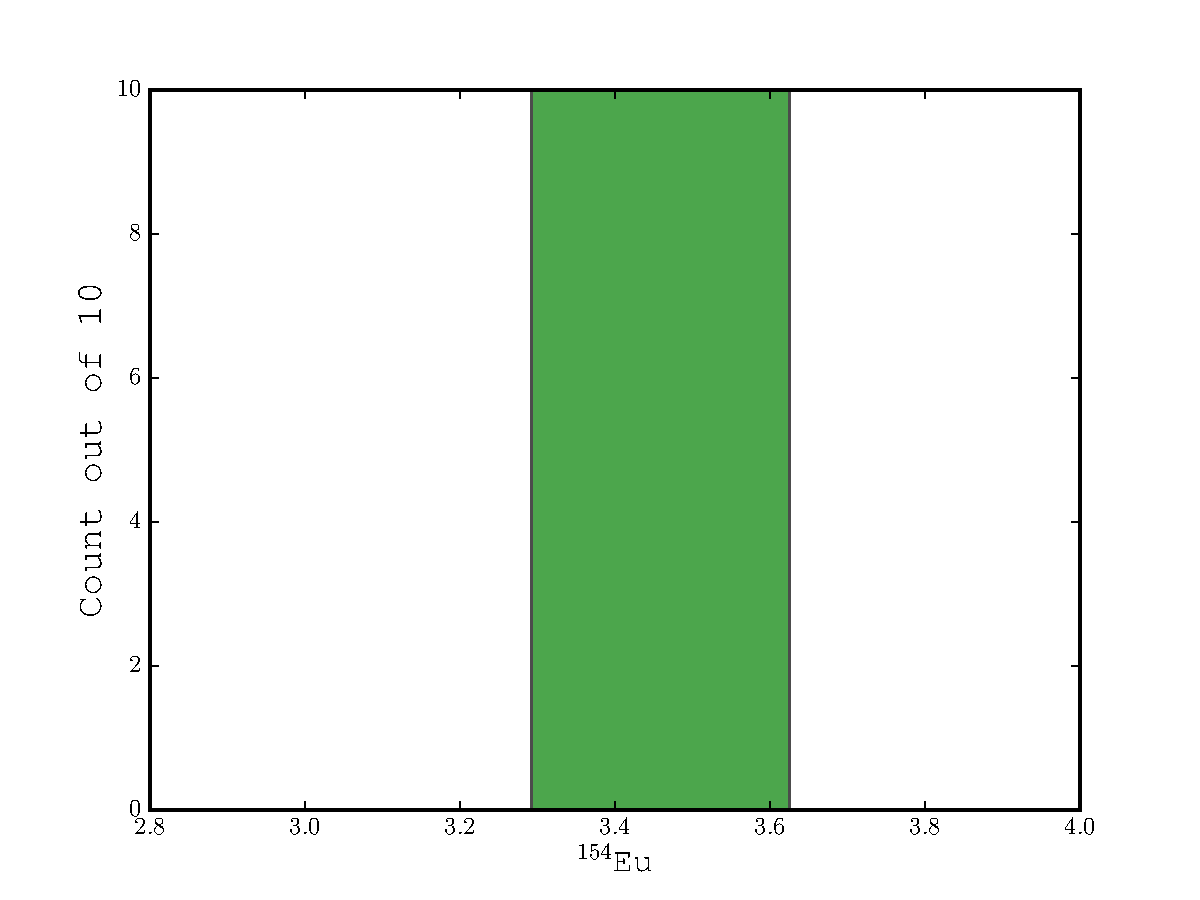
\includegraphics[width=0.77\columnwidth]{../Origen2/PLOTS/EU154Post_HIST.pdf}
      \vspace{-5mm}
      \caption{Histogram of QOI \tss{154}Eu}
      \label{fig:POSTHISTEu154}
    \end{center}
  \end{figure}

    \begin{figure}[H]
    \begin{center}
      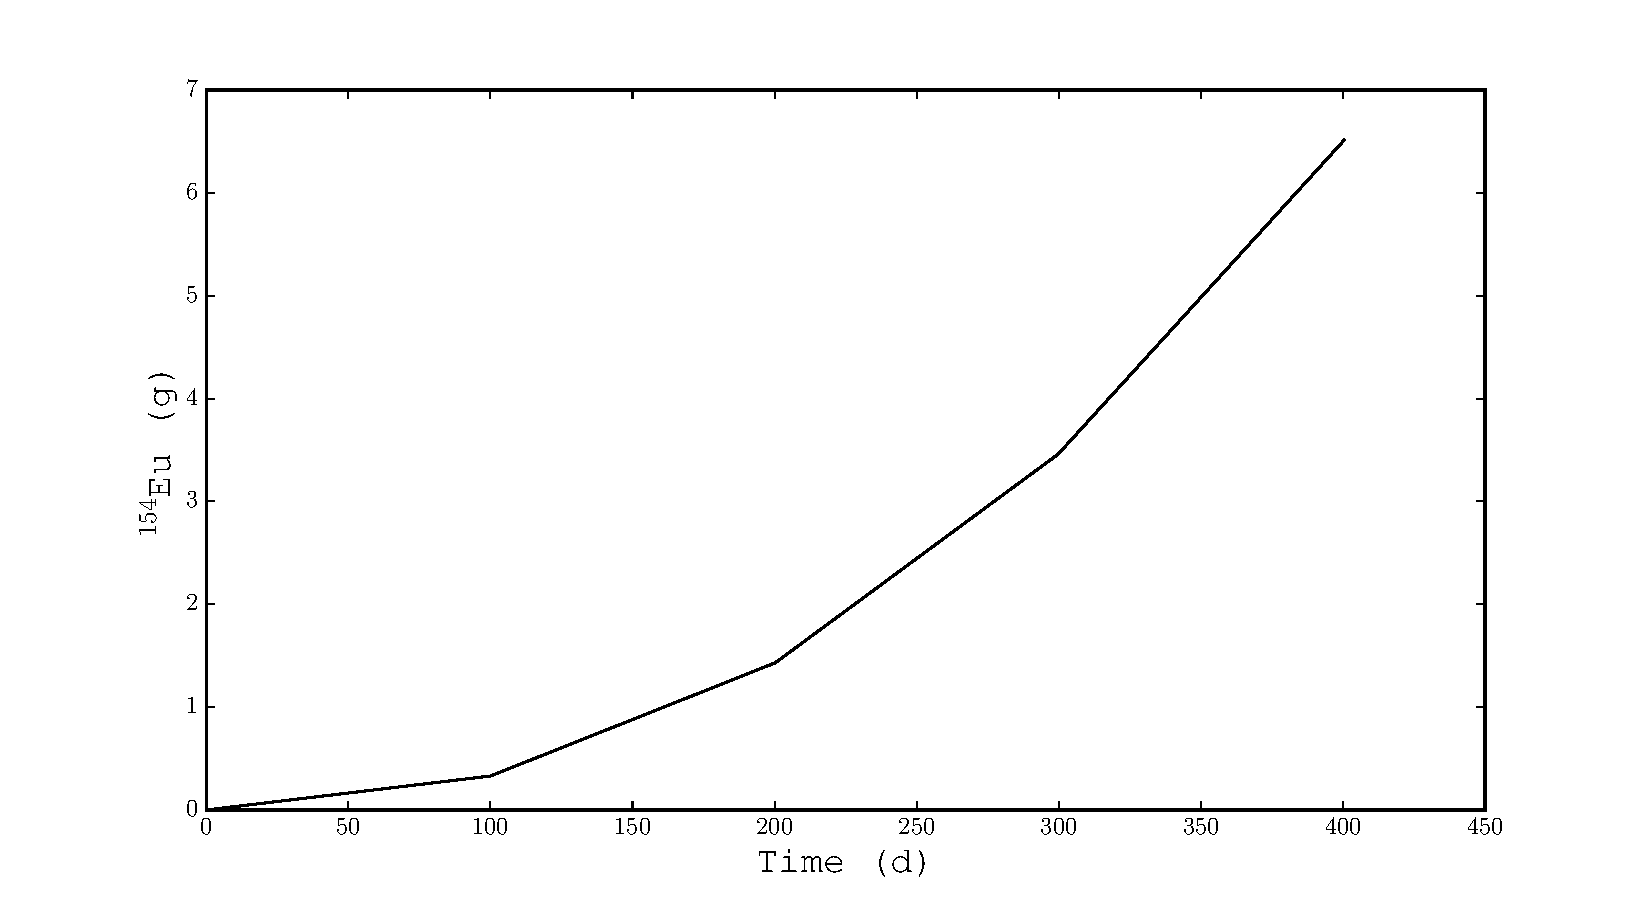
\includegraphics[width=0.77\columnwidth]{../Origen2/PLOTS/EU154Post_XY.pdf}
      \vspace{-5mm}
      \caption{XY plot of QOI \tss{154}Eu}
      \label{fig:POSTXYEu154}
    \end{center}
  \end{figure}

  \begin{figure}[H]
    \begin{center}
      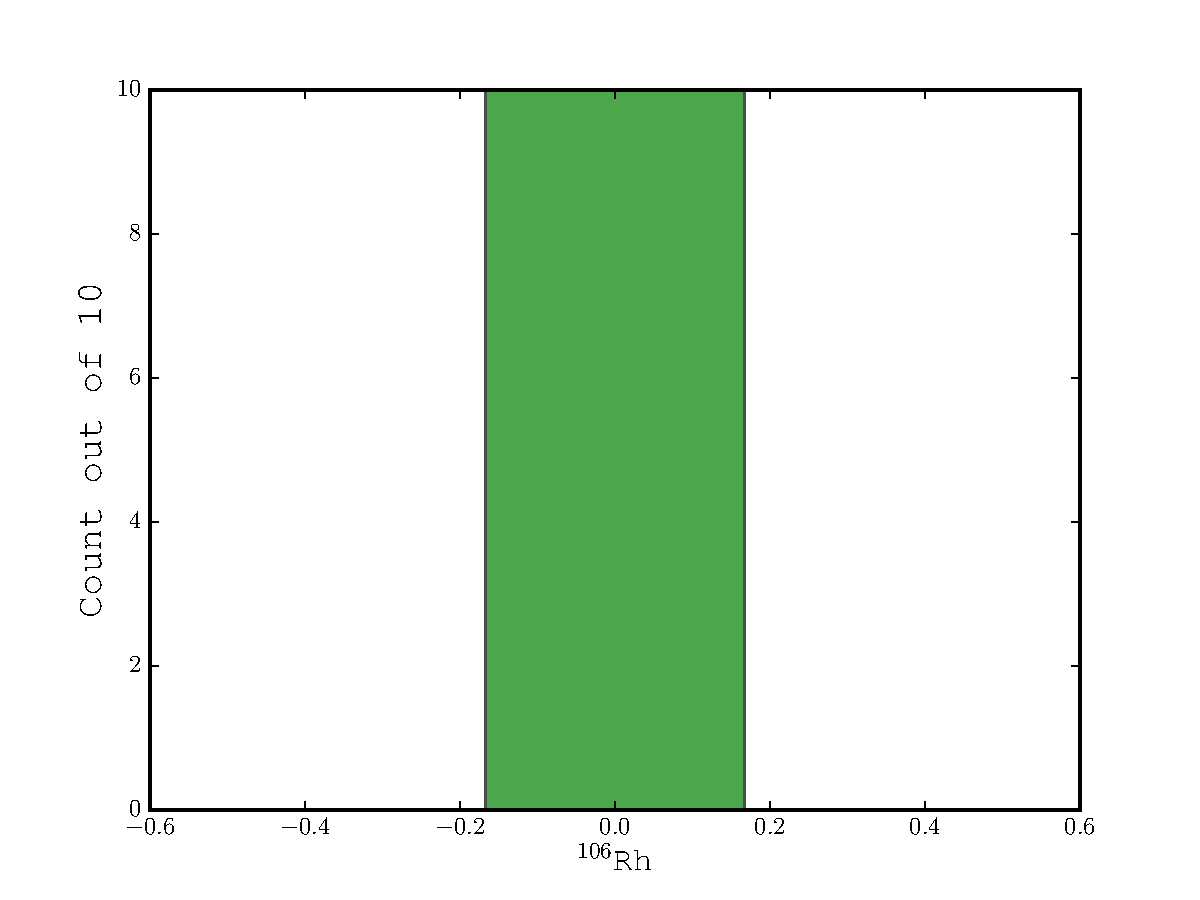
\includegraphics[width=0.77\columnwidth]{../Origen2/PLOTS/RH106Post_HIST.pdf}
      \vspace{-5mm}
      \caption{Histogram of QOI \tss{106}Rh}
      \label{fig:POSTHISTRh106}
    \end{center}
  \end{figure}

    \begin{figure}[H]
    \begin{center}
      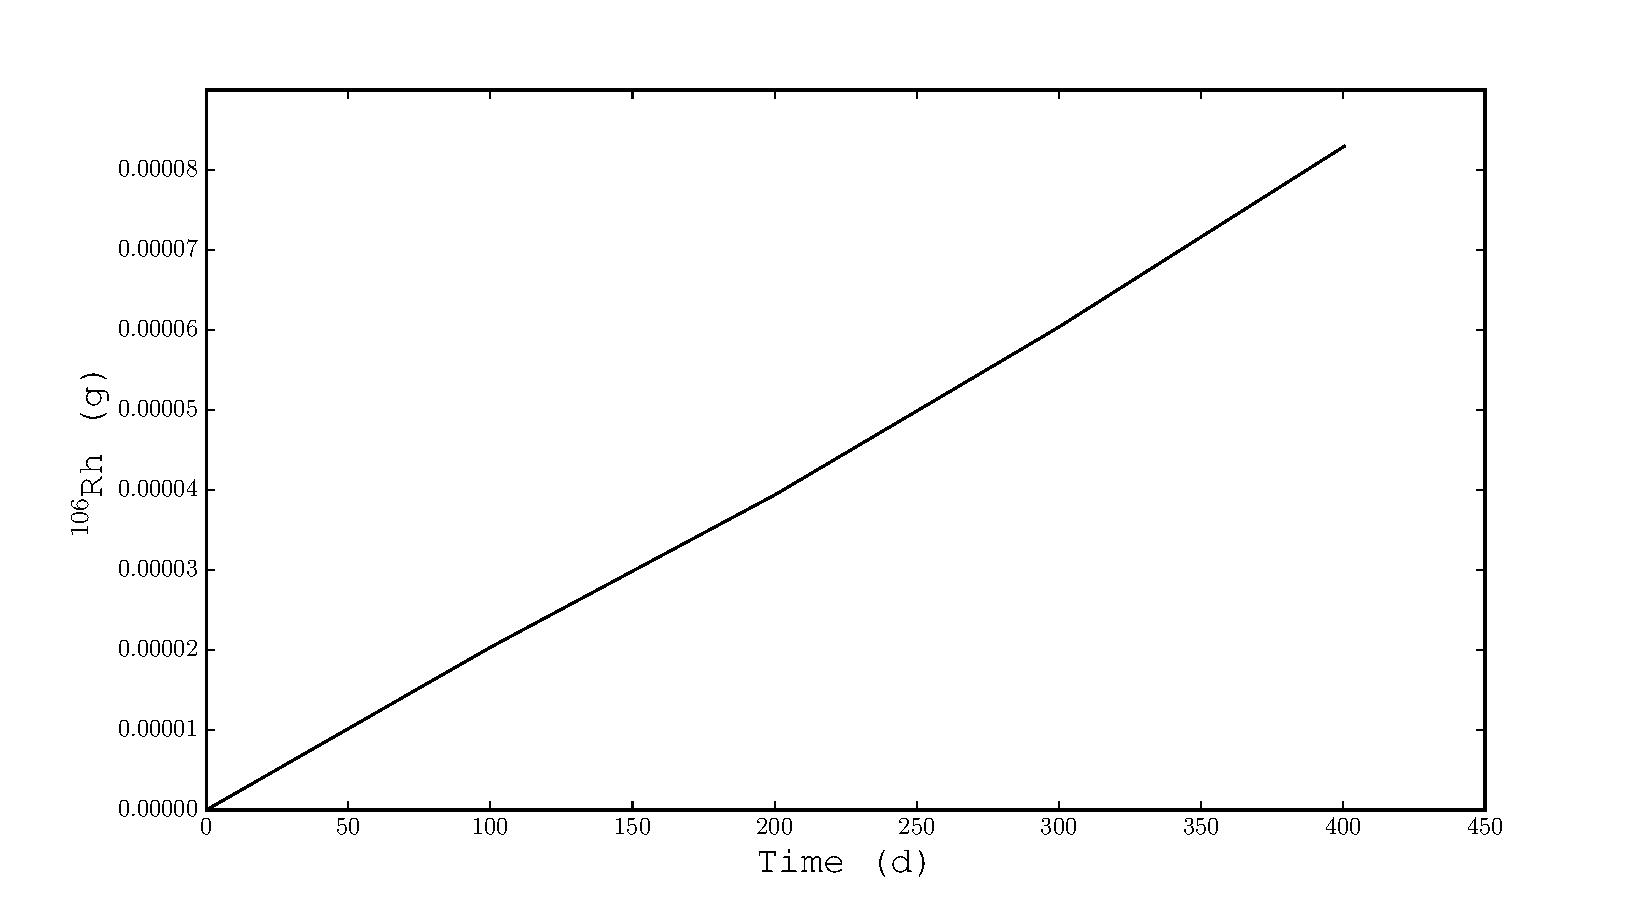
\includegraphics[width=0.77\columnwidth]{../Origen2/PLOTS/RH106Post_XY.pdf}
      \vspace{-5mm}
      \caption{XY plot of QOI \tss{106}Rh}
      \label{fig:POSTXYRh106}
    \end{center}
  \end{figure}

  \begin{figure}[H]
    \begin{center}
      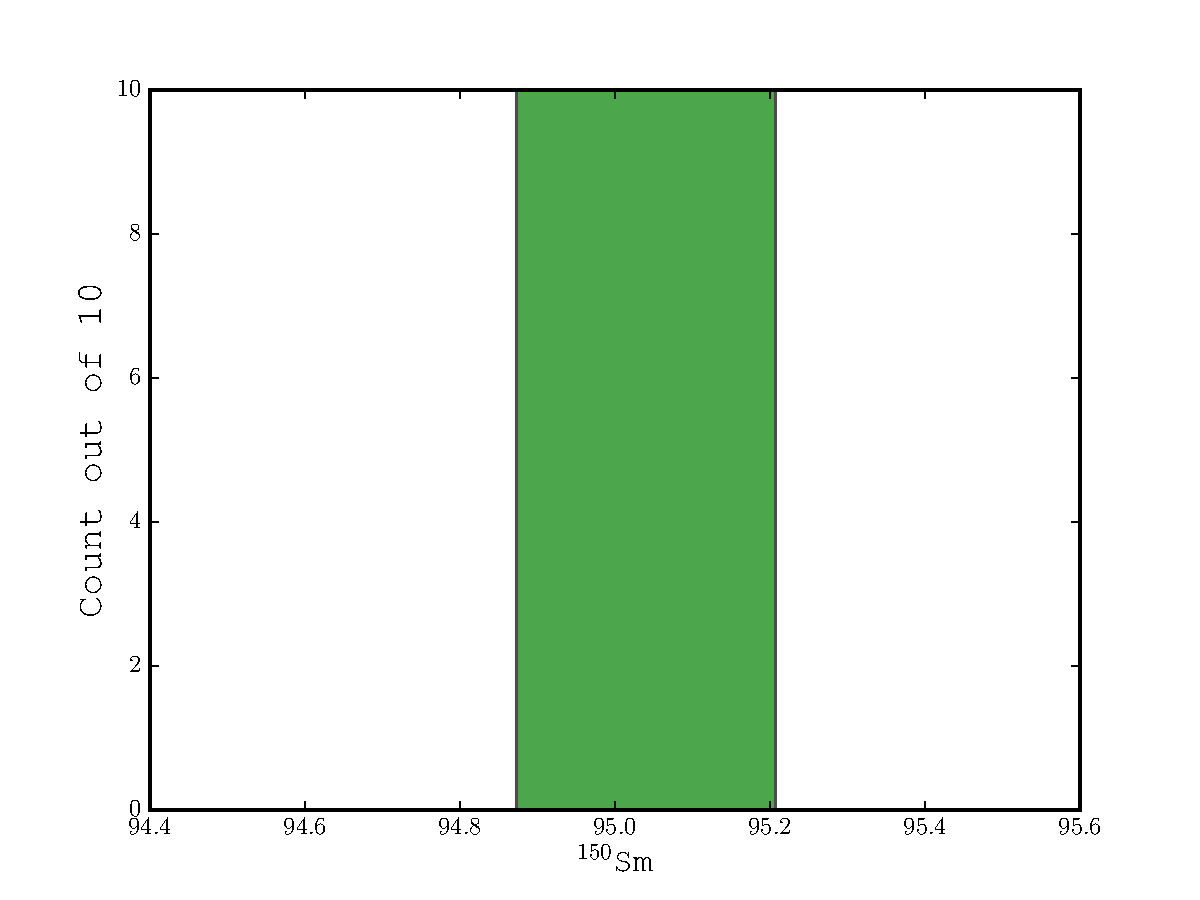
\includegraphics[width=0.77\columnwidth]{../Origen2/PLOTS/SM150Post_HIST.pdf}
      \vspace{-5mm}
      \caption{Histogram of QOI \tss{150}Sm}
      \label{fig:POSTHISTSm150}
    \end{center}
  \end{figure}

    \begin{figure}[H]
    \begin{center}
      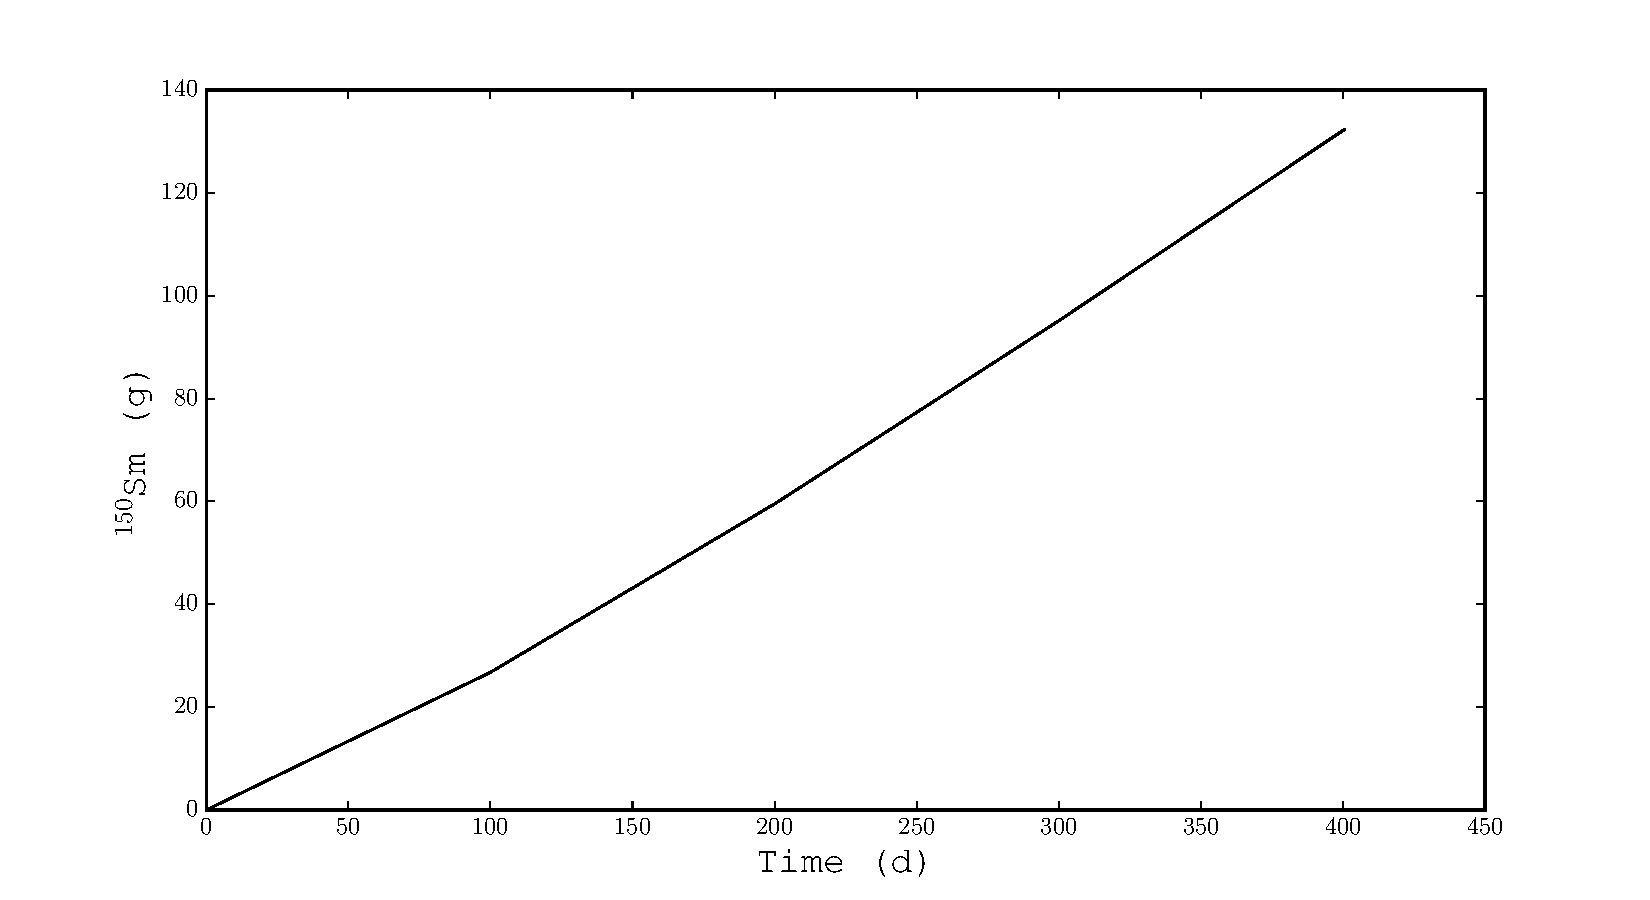
\includegraphics[width=0.77\columnwidth]{../Origen2/PLOTS/SM150Post_XY.pdf}
      \vspace{-5mm}
      \caption{XY plot of QOI \tss{150}Sm}
      \label{fig:POSTXYSm150}
    \end{center}
  \end{figure}

  \begin{figure}[H]
    \begin{center}
      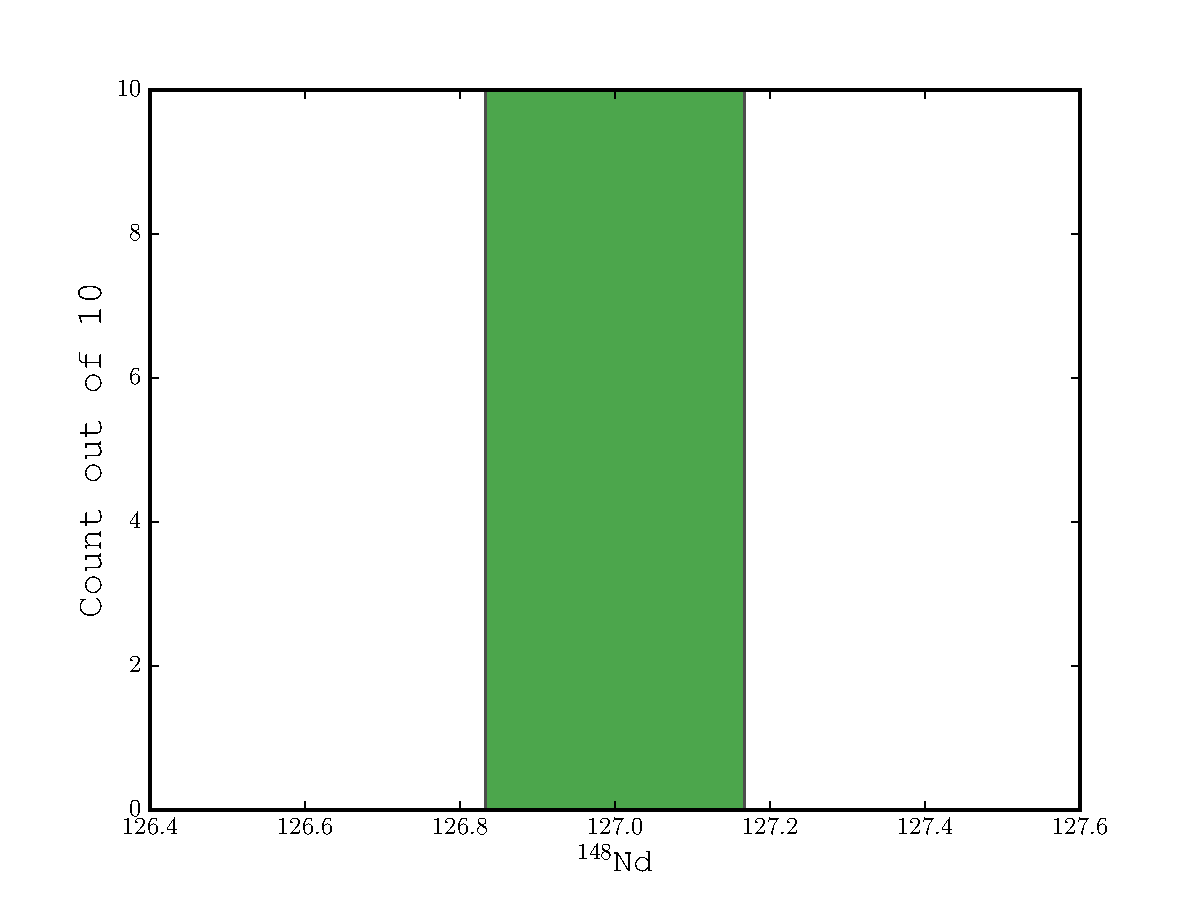
\includegraphics[width=0.77\columnwidth]{../Origen2/PLOTS/ND148Post_HIST.pdf}
      \vspace{-5mm}
      \caption{Histogram of QOI \tss{148}Nd}
      \label{fig:POSTHISTNd148}
    \end{center}
  \end{figure}

    \begin{figure}[H]
    \begin{center}
      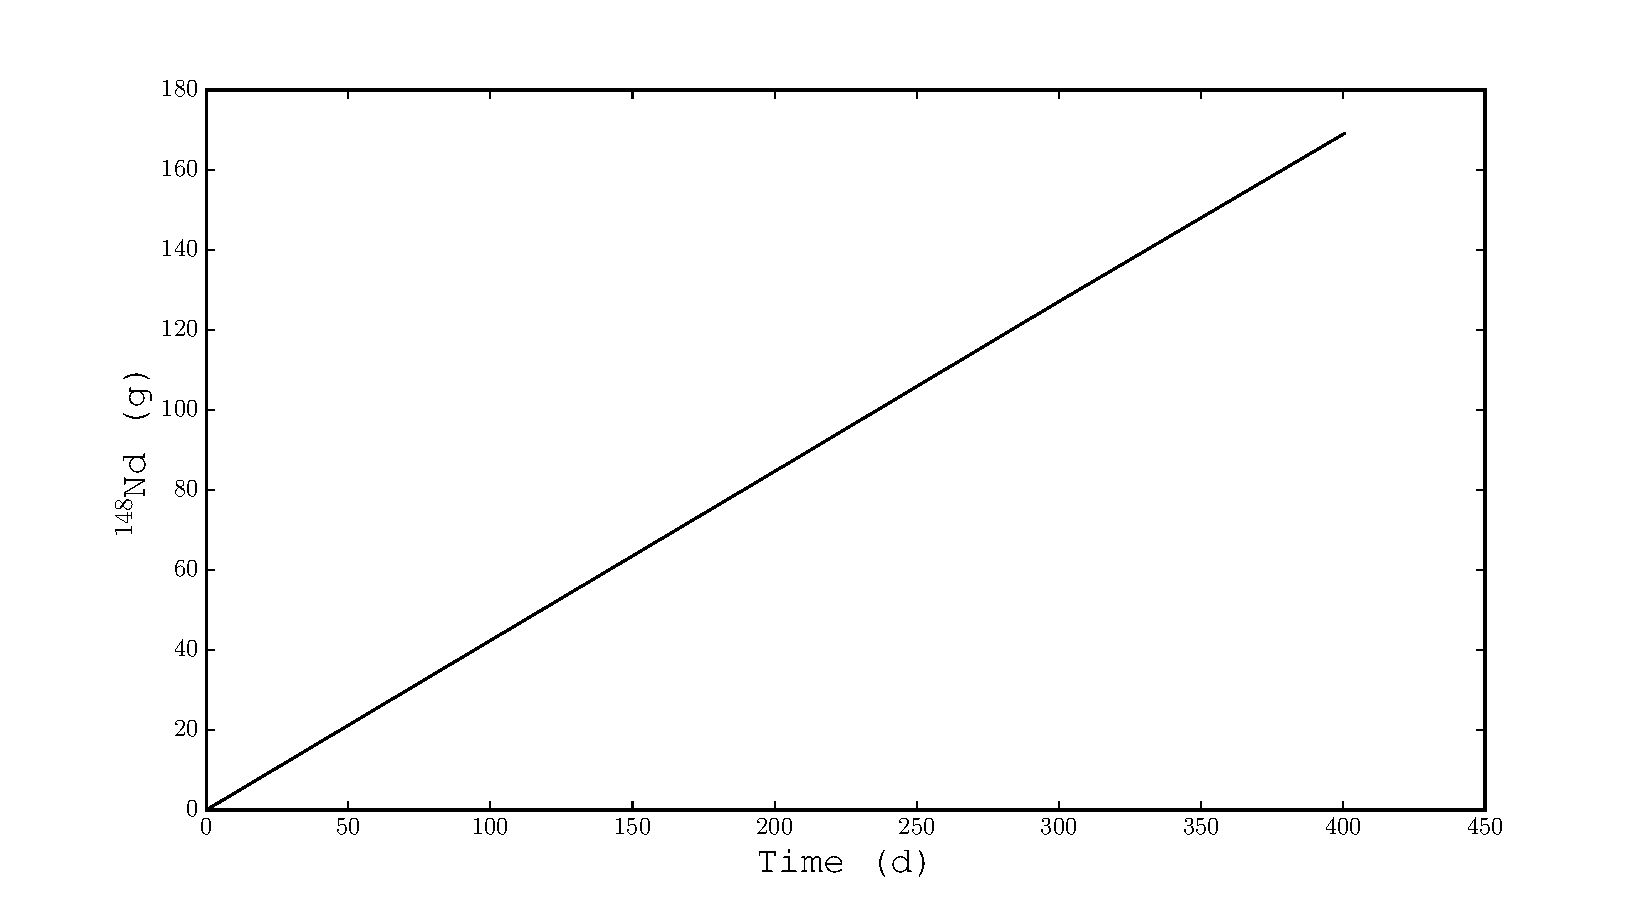
\includegraphics[width=0.77\columnwidth]{../Origen2/PLOTS/ND148Post_XY.pdf}
      \vspace{-5mm}
      \caption{XY plot of QOI \tss{148}Nd}
      \label{fig:POSTXYNd148}
    \end{center}
  \end{figure}

  \begin{figure}[H]
    \begin{center}
      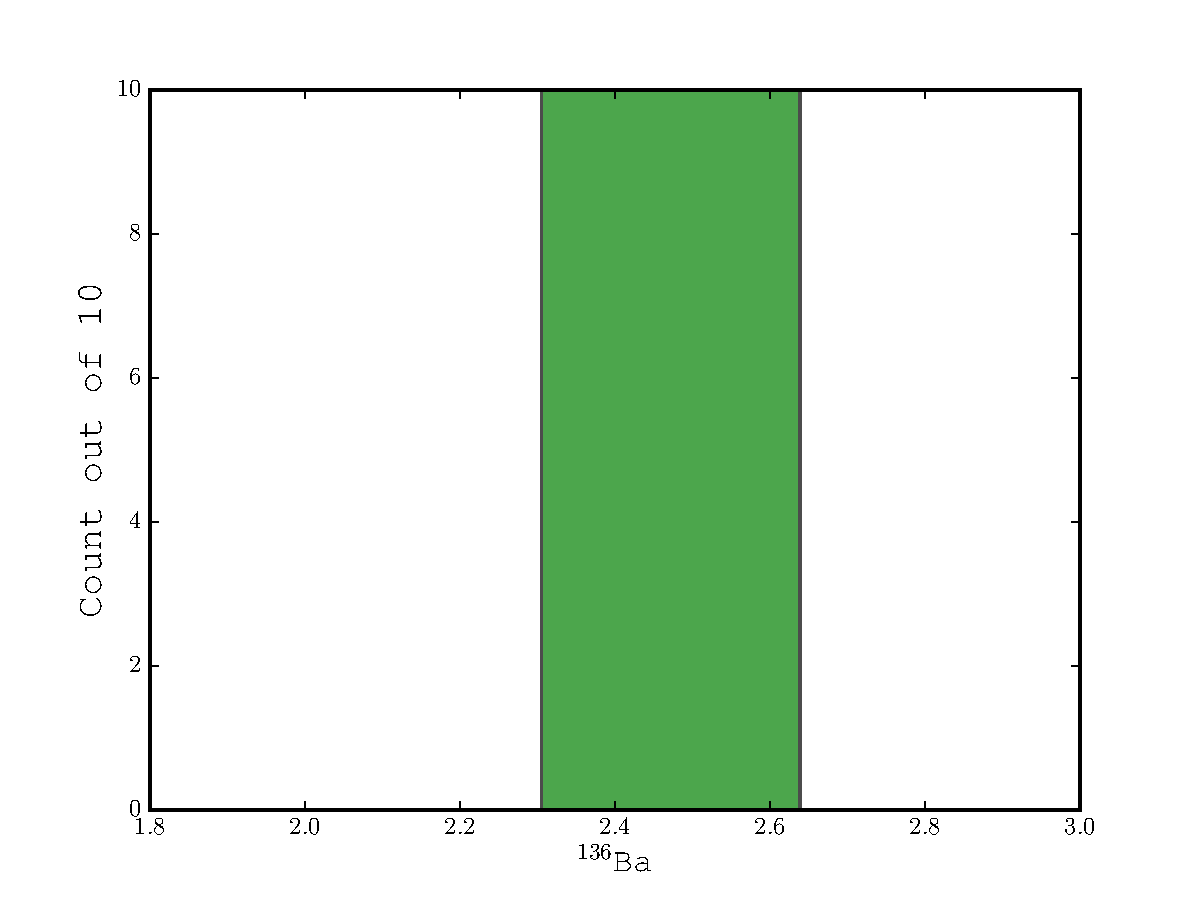
\includegraphics[width=0.77\columnwidth]{../Origen2/PLOTS/BA136Post_HIST.pdf}
      \vspace{-5mm}
      \caption{Histogram of QOI \tss{136}Ba}
      \label{fig:POSTHISTBa136}
    \end{center}
  \end{figure}

    \begin{figure}[H]
    \begin{center}
      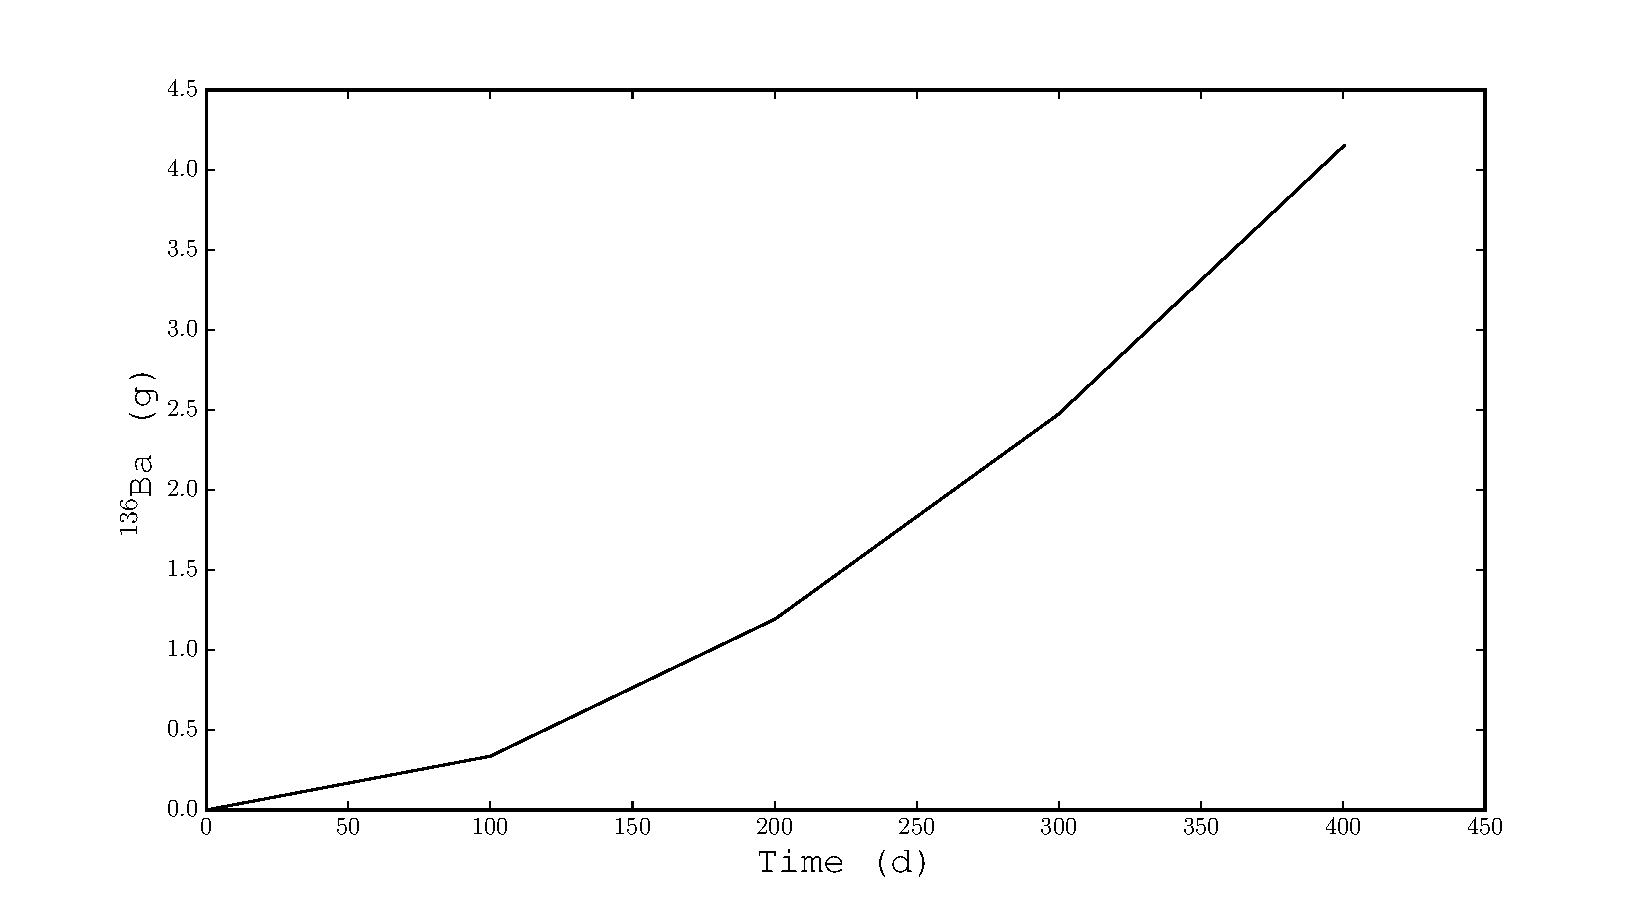
\includegraphics[width=0.77\columnwidth]{../Origen2/PLOTS/BA136Post_XY.pdf}
      \vspace{-5mm}
      \caption{XY plot of QOI \tss{136}Ba}
      \label{fig:POSTXYBa136}
    \end{center}
  \end{figure}

  \begin{figure}[H]
    \begin{center}
      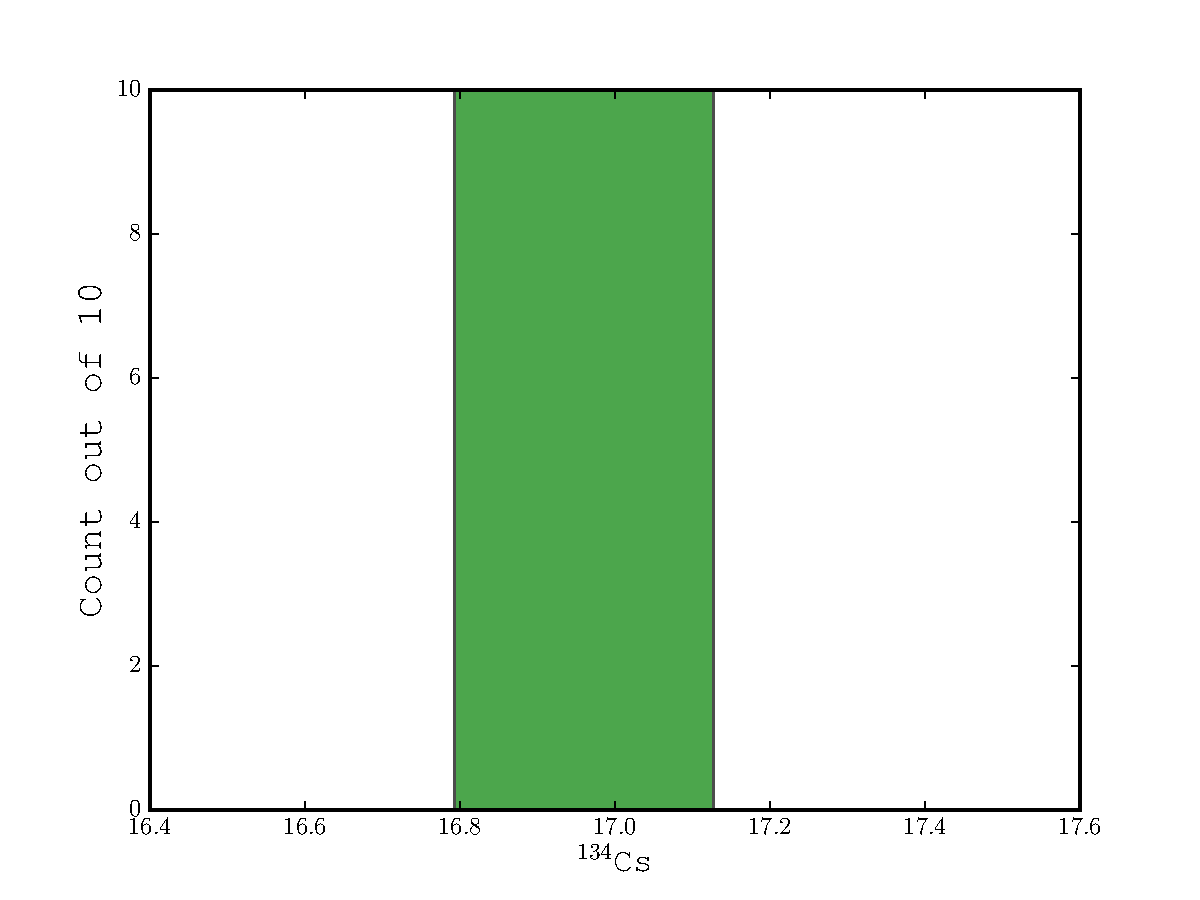
\includegraphics[width=0.77\columnwidth]{../Origen2/PLOTS/CS134Post_HIST.pdf}
      \vspace{-5mm}
      \caption{Histogram of QOI \tss{134}Cs}
      \label{fig:POSTHISTBa136}
    \end{center}
  \end{figure}

    \begin{figure}[H]
    \begin{center}
      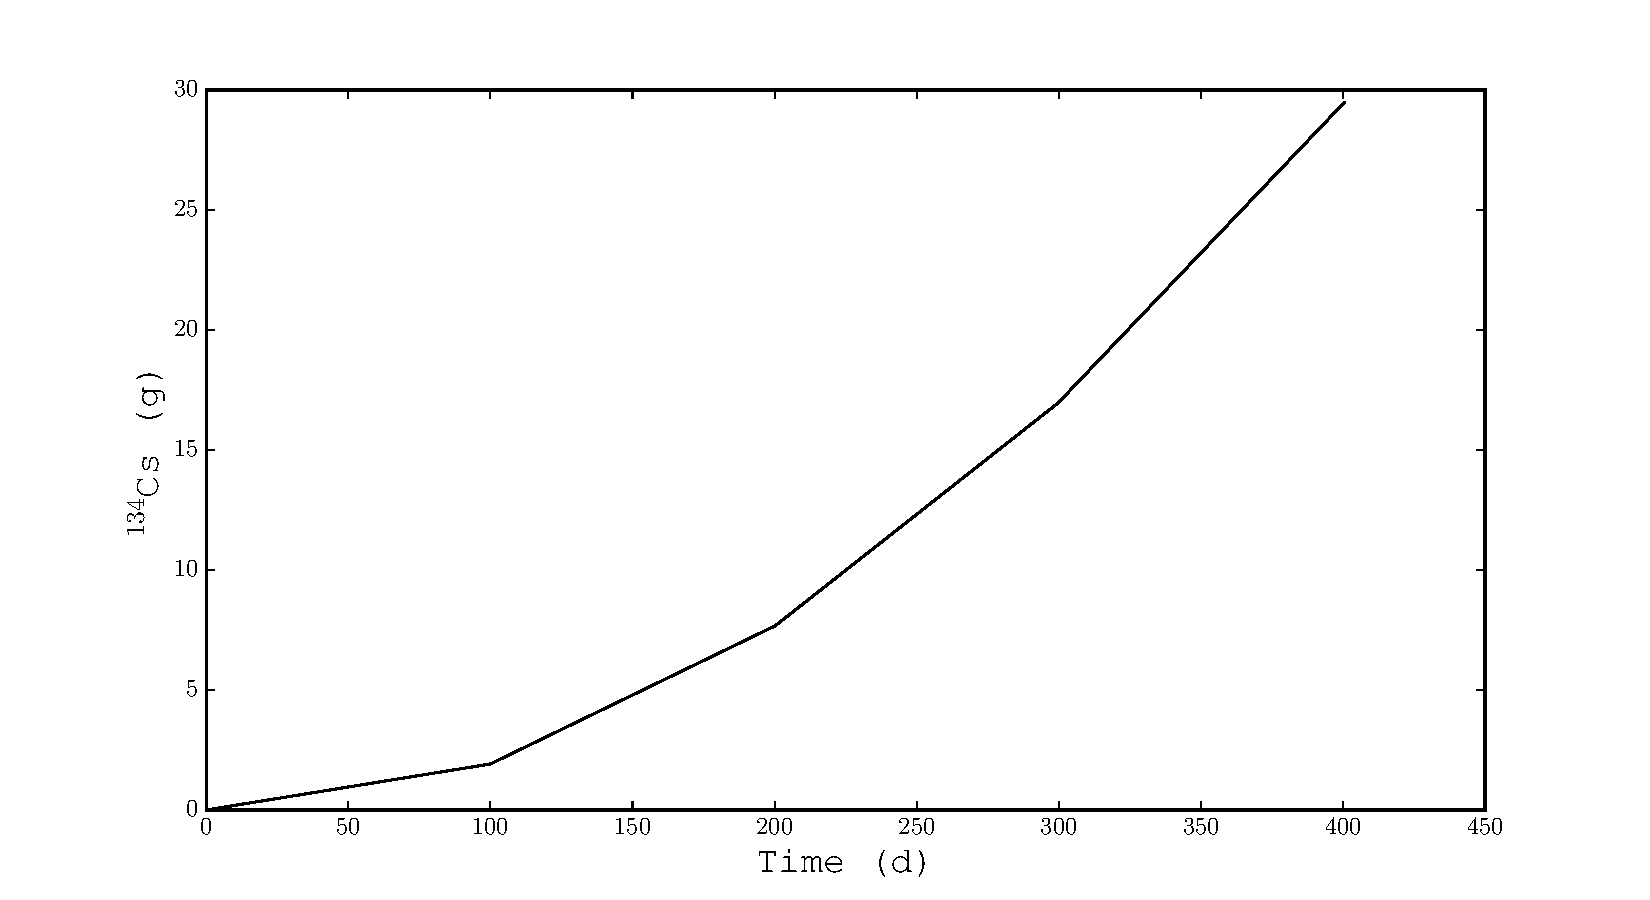
\includegraphics[width=0.77\columnwidth]{../Origen2/PLOTS/CS134Post_XY.pdf}
      \vspace{-5mm}
      \caption{XY plot of QOI \tss{134}Cs}
      \label{fig:POSTXYCs134}
    \end{center}
  \end{figure}


I apologize for the wall of graphs. I left some out.
%------------------------------------------------------------
%	Prediction
%------------------------------------------------------------

\section{Conclusions}

There was an unexpectedly large amount of error in the
one group cross sections, but currently there is no variation
in the output, even when I change the cross section by a
factor of over 1000, I don't think ORIGEN is taking up
what I am laying down.

%-----------------------------------------------------------
\bibliography{references}
\bibliographystyle{plain}


\end{document}
